\documentclass[12pt]{article}
\usepackage{fullpage,graphicx,psfrag,url,ar,rotating,float}
\usepackage[small,bf]{caption}
\usepackage{amsmath,amssymb,enumitem,bbm,subcaption,multirow}
\setlength{\captionmargin}{20pt}
\setlist[enumerate]{label=(\roman*)}

\title{\Large{AA274 (Winter 2017-18): Problem Set 1}}
\author{Anqi Fu}

\begin{document}
\maketitle

\section{Optimal Control}
\begin{enumerate}
	\item Let $\mathbf{x} = (x,y,\theta)$ denote the robot state and $\mathbf{u} = (V,\omega)$ be the robot control inputs. Our optimal control problem is
	\begin{equation}\label{eqn:1_1_opt}
		\begin{array}{cc}
		\underset{(V,\omega)}{\mbox{minimize}} & \int_0^{t_f} [\lambda + V(t)^2 + \omega(t)^2]dt \\
		\mbox{subject to} & \dot x(t) = V\cos(\theta(t)), \\
		& \dot y(t) = V\sin(\theta(t)), \\
		& \dot \theta(t) = \omega(t), \\
		& |V(t)| \leq 0.5, \\
		& |\omega(t)| \leq 1.0.
		\end{array}
	\end{equation}
	with initial and final conditions
	\begin{align*}
		&x(0) = 0, \quad y(0) = 0, \quad \theta(0) = -\pi/2, \\
		&x(t_f) = 5, \quad y(t_f) = 5, \quad \theta(t_f) = -\pi/2.
	\end{align*}
	Here $\lambda \in \mathbb{R}_+$ is a weighting factor and $t_f$ is free. The Hamiltonian is
	\[
		H(t) = \lambda + V(t)^2 + \omega(t)^2 + p_1(t)V(t)\cos(\theta(t)) + p_2(t)V(t)\sin(\theta(t)) + p_3(t)\omega(t)
	\]
	where $\mathbf{p} = (p_1,p_2,p_3)$ are the Lagrange multipliers associated with $\dot{\mathbf{x}} = (\dot x, \dot y, \dot \theta)$. Our optimality conditions are
	\begin{align}\label{eqn:1_1_cond}
	\begin{split}
		\left(\begin{array}{c}
		\dot x^*(t) \\
		\dot y^*(t) \\
		\dot \theta^*(t)
		\end{array}\right) &=
		\left(\begin{array}{c}
		V^*(t)\cos(\theta^*(t)) \\
		V^*(t)\sin(\theta^*(t)) \\
		\omega^*(t)
		\end{array}\right) \\	
		\left(\begin{array}{c}
		\dot p_1^*(t) \\
		\dot p_2^*(t) \\
		\dot p_3^*(t)
		\end{array}\right) &=
		\left(\begin{array}{c}
		0 \\
		0 \\
		p_1^*(t)V^*(t)\sin(\theta^*(t)) - p_2^*(t)V^*(t)\cos(\theta^*(t))
		\end{array}\right)
	\end{split}
	\end{align}
	with the additional constraint (for the control inequality constraints)
	\begin{align}\label{eqn:1_1_ineq}
	\begin{split}
		&V^*(t)^2 + \omega^*(t)^2 + p_1^*(t)V^*(t)\cos(\theta^*(t)) + p_2^*(t)V^*(t)\sin(\theta^*(t)) + p_3^*(t)\omega^*(t) \\
	\leq \; &V(t)^2 + \omega(t)^2 + p_1^*(t)V(t)\cos(\theta^*(t)) + p_2^*(t)V(t)\sin(\theta^*(t)) + p_3^*(t)\omega(t)
	\end{split}
	\end{align}
	for all $(V(t), \omega(t)) \in \mathbb{R}^2$. Since $t_f$ is free and $\mathbf{x}(t_f)$ is fixed, the boundary conditions amount to
	\begin{align*}
		&x^*(0) = 0, \quad y^*(0) = 0, \quad \theta^*(0) = -\pi/2, \\
		&x^*(t_f) = 5, \quad y^*(t_f) = 5, \quad \theta^*(t_f) = -\pi/2, \\
		&\lambda + V^*(t_f)^2 + \omega^*(t_f)^2 + p_1^*(t_f)V^*(t_f)\cos(\theta^*(t_f)) + p_2^*(t_f)V^*(t_f)\sin(\theta^*(t_f)) + p_3^*(t_f)\omega^*(t_f) \\
		= \; &\lambda + V^*(t_f)^2 + \omega^*(t_f)^2 - p_2^*(t_f)V^*(t_f) + p_3^*(t_f)\omega^*(t_f) = 0.
	\end{align*}
	We make two modifications in order to solve this problem. First, we ignore the control inequality constraints and manually vary $\lambda$. This means that (\ref{eqn:1_1_ineq}) is replaced with
	\begin{align}\label{eqn:1_1_Vom}
	\begin{split}
		\left(\begin{array}{c}
		0 \\
		0
		\end{array}\right) &=
		\left(\begin{array}{c}
		2V^*(t) + p_1^*(t)\cos(\theta^*(t)) + p_2^*(t)\sin(\theta^*(t)) \\
		2\omega^*(t) + p_3^*(t)
		\end{array}\right) \\
		\Rightarrow \left(\begin{array}{c}
		V^*(t) \\
		\omega^*(t)
		\end{array}\right) &=
		-\frac{1}{2}\left(\begin{array}{c}
		p_1^*(t)\cos(\theta^*(t)) + p_2^*(t)\sin(\theta^*(t)) \\
		p_3^*(t)
		\end{array}\right)
	\end{split}
	\end{align}
	Second, we use a change of variables to reformulate the BVP: we rescale the time to $\tau = \frac{t}{t_f} \in [0,1]$ so derivatives become $\frac{d}{d\tau} := t_f\frac{d}{dt}$, then introduce a dummy state variable $r$ that corresponds to $t_f$ with dynamic $\dot r = 0$ and replace all instances of $t_f$ with $r$. Let $\mathbf{z} = (x, y, \theta, p_1, p_2, p_3, r)$ denote the augmented state vector, then $\frac{d\mathbf{z}}{dt} = \frac{1}{t_f}\frac{d\mathbf{z}}{d\tau} = \frac{1}{r}\frac{d\mathbf{z}}{d\tau}$ and (\ref{eqn:1_1_cond}) becomes
	\begin{equation}\label{eqn:1_1_bvp_opt}
		\frac{d\mathbf{z}}{d\tau} =
		z_7\left(\begin{array}{c}
		V\cos(z_3) \\
		V\sin(z_3) \\
		\omega \\
		0 \\
		0 \\
		V(z_4\sin(z_3) - z_5\cos(z_3)) \\
		0
		\end{array}\right)
	\end{equation}
	with boundary conditions
	\begin{align}\label{eqn:1_1_bvp_bc}
	\begin{split}
		&z_1(0) = 0, \quad z_2(0) = 0, \quad z_3(0) = -\pi/2 \\
		&z_1(1) = 5, \quad z_2(1) = 5, \quad z_3(1) = -\pi/2 \\
		&\lambda + V(1)^2 + \omega(1)^2 - z_5(1)V(1) + z_6(1)\omega(1) = 0
	\end{split}
	\end{align}
	where we have used (\ref{eqn:1_1_Vom}) to define
	\begin{equation}\label{eqn:1_1_bvp_Vom}
		\left(\begin{array}{c}
		V \\
		\omega
		\end{array}\right) :=
		-\frac{1}{2}\left(\begin{array}{c}
		z_4\cos(z_3) + z_5\sin(z_3) \\
		z_6
		\end{array}\right)
	\end{equation}
	\item See submitted code.
	\item By choosing the largest feasible $\lambda$, we are solving the control problem with the smallest feasible $t_f$, i.e., our optimal control functions drive the unicycle to its final waypoint in the shortest possible time. This can be seen by separating the objective into
	\[
		J = \int_0^{t_f} [\lambda + V(t)^2 + \omega(t)^2]dt = \lambda t_f + \int_0^{t_f} [V(t)^2 + \omega(t)^2]dt.
	\]
	Here $\lambda \geq 0$ acts like a regularization weight: a larger value of $\lambda$ upweights $t_f$ relative to the rest of the objective, which means (since we are minimizing $J$) that we place more importance on reducing $t_f$ in the optimization. Selecting the largest feasible $\lambda$ makes sense because in general, we prefer to travel between the initial and final waypoints as quickly as possible.
	\item See submitted code. With $\lambda = 0.238$ and solution guess $\mathbf{z}_0 = (0, 0, -\pi/2, 1, 1, 0, 10)$, we get $V < 0$ and the robot backs up from $(0,0)$ to $(5,5)$. Its trajectory and control histories are shown below.
	\begin{figure}[H]
		\centering
		\title{\bf Trajectory $(x(t), y(t))$)}
		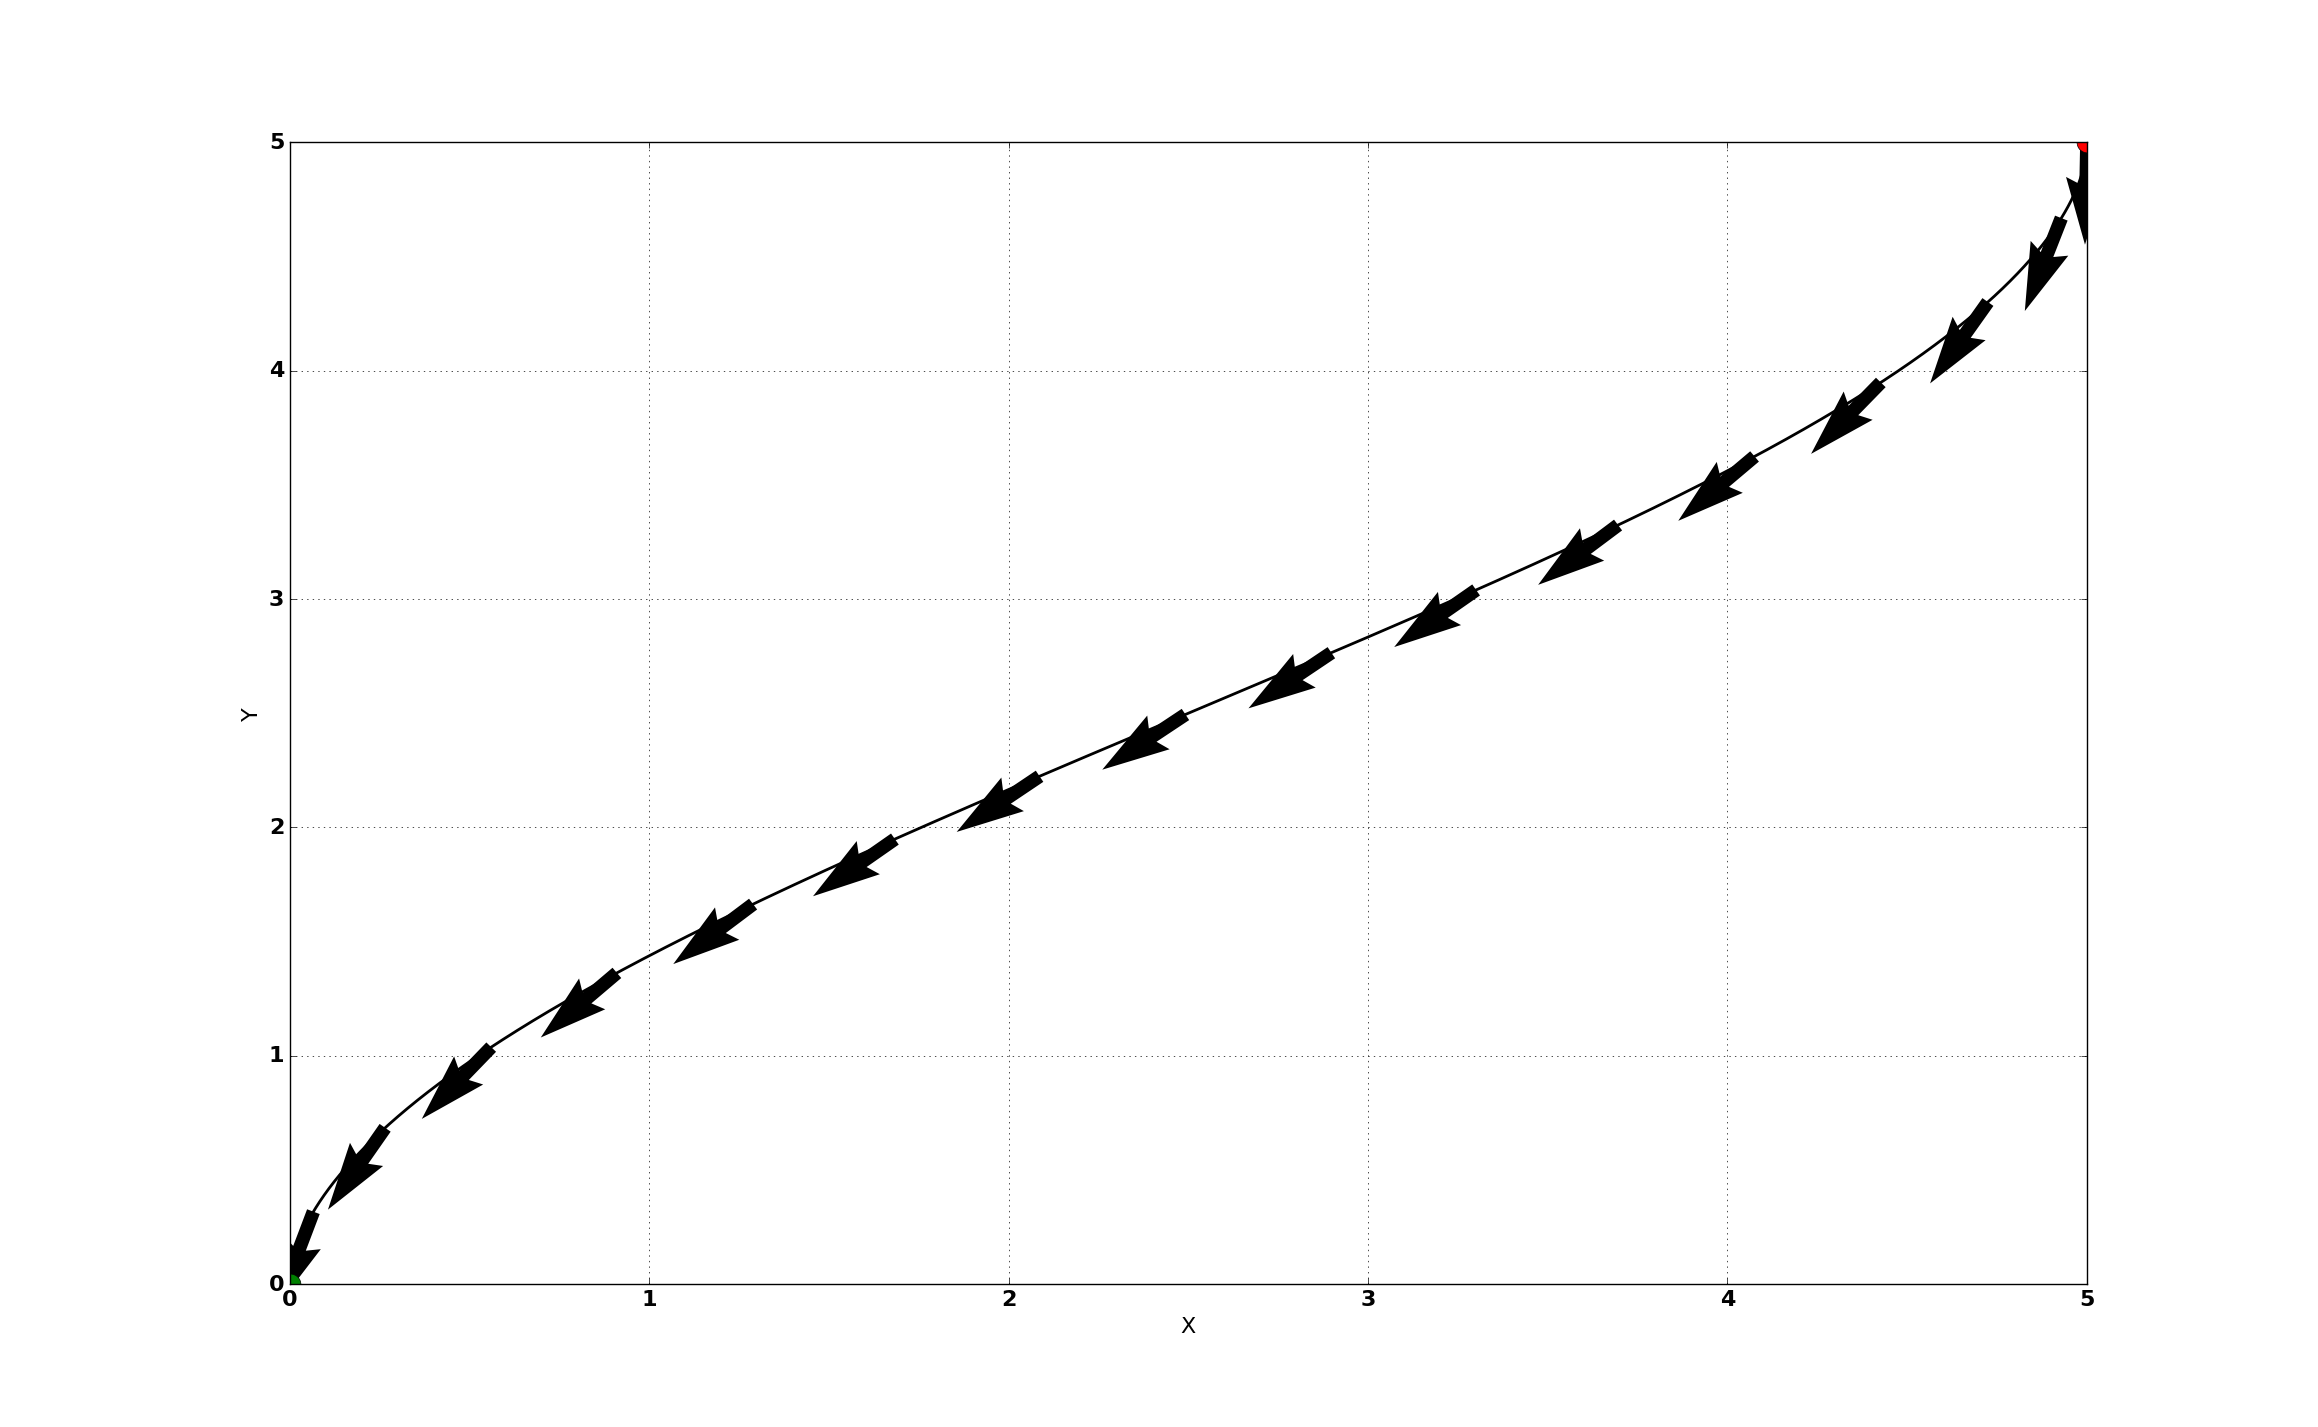
\includegraphics[width=\textwidth]{../Figures/hw1_1_iv_a.png}
	\end{figure}
	\begin{figure}[H]
		\centering
		\title{\bf History of $V$ and $\omega$}
		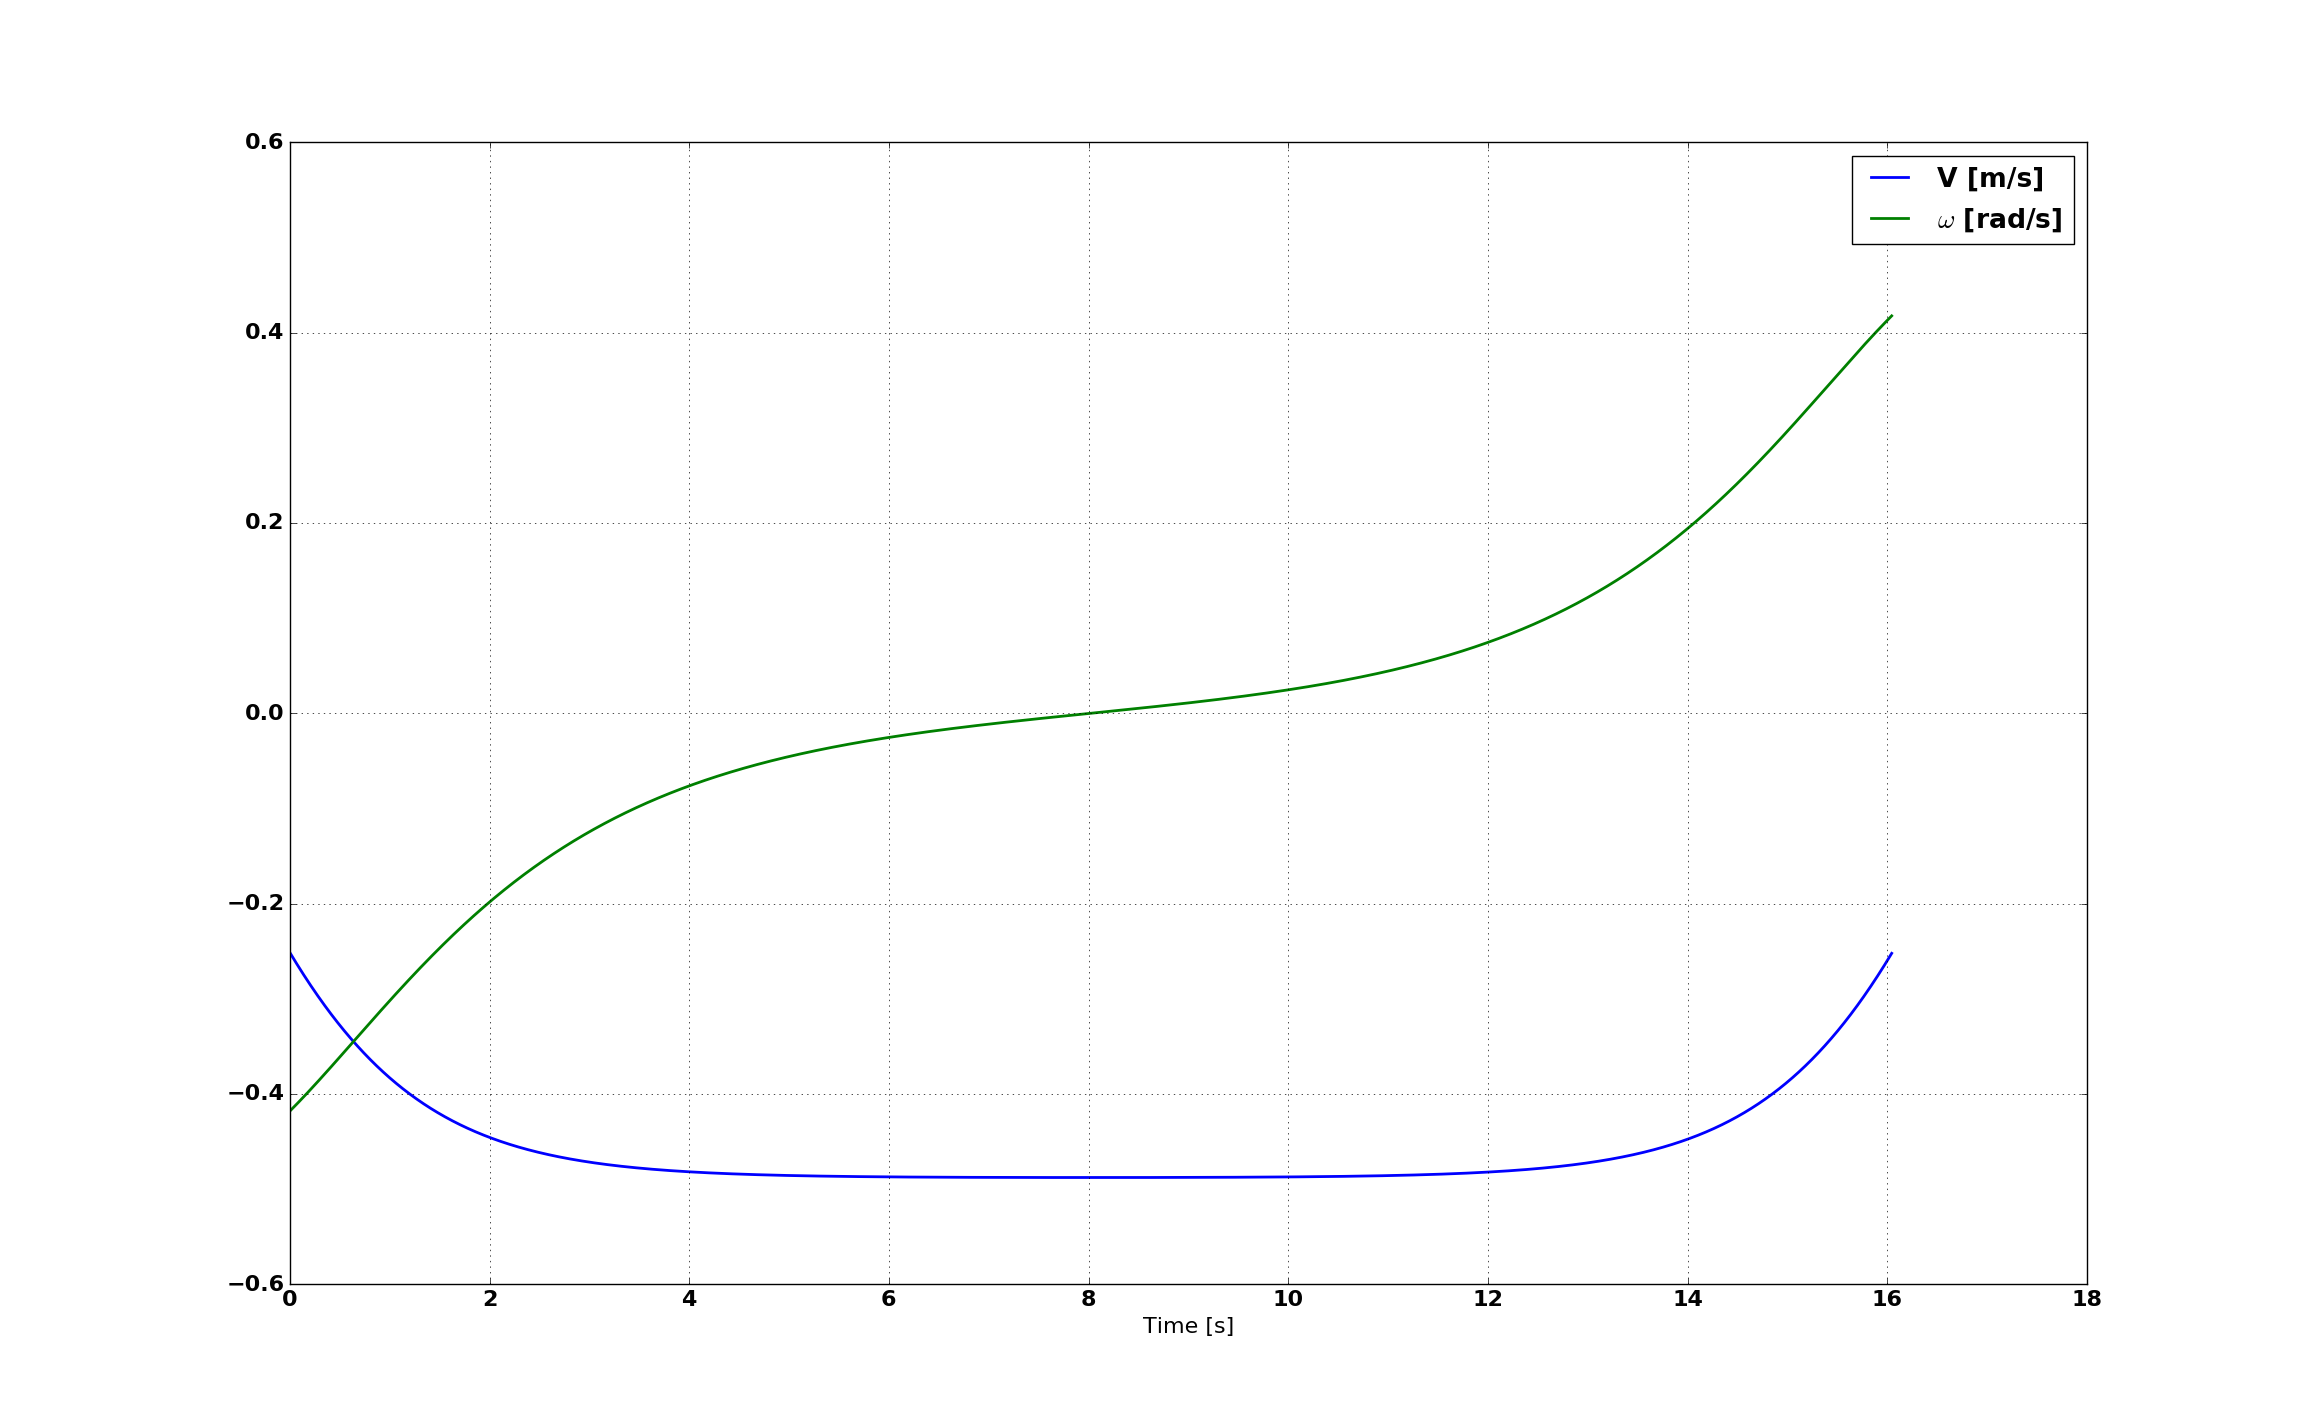
\includegraphics[width=\textwidth]{../Figures/hw1_1_iv_b.png}
	\end{figure}
	\item See submitted code.
	\begin{figure}[H]
		\centering
		\title{\bf Trajectory $(x(t), y(t))$)}
		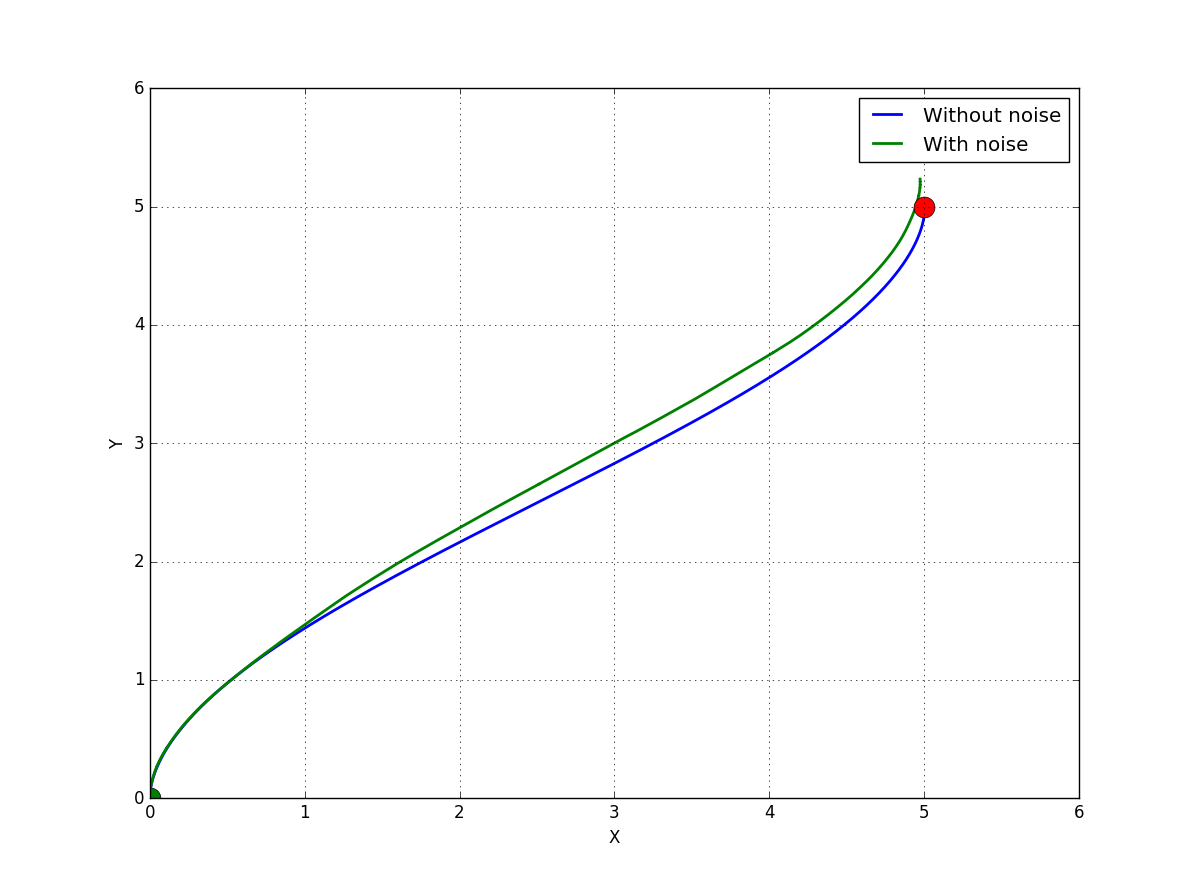
\includegraphics[width=\textwidth]{../Figures/hw1_1_v_traj.png}
	\end{figure}
	\begin{figure}[H]
		\centering
		\title{\bf History of $V$ and $\omega$}
		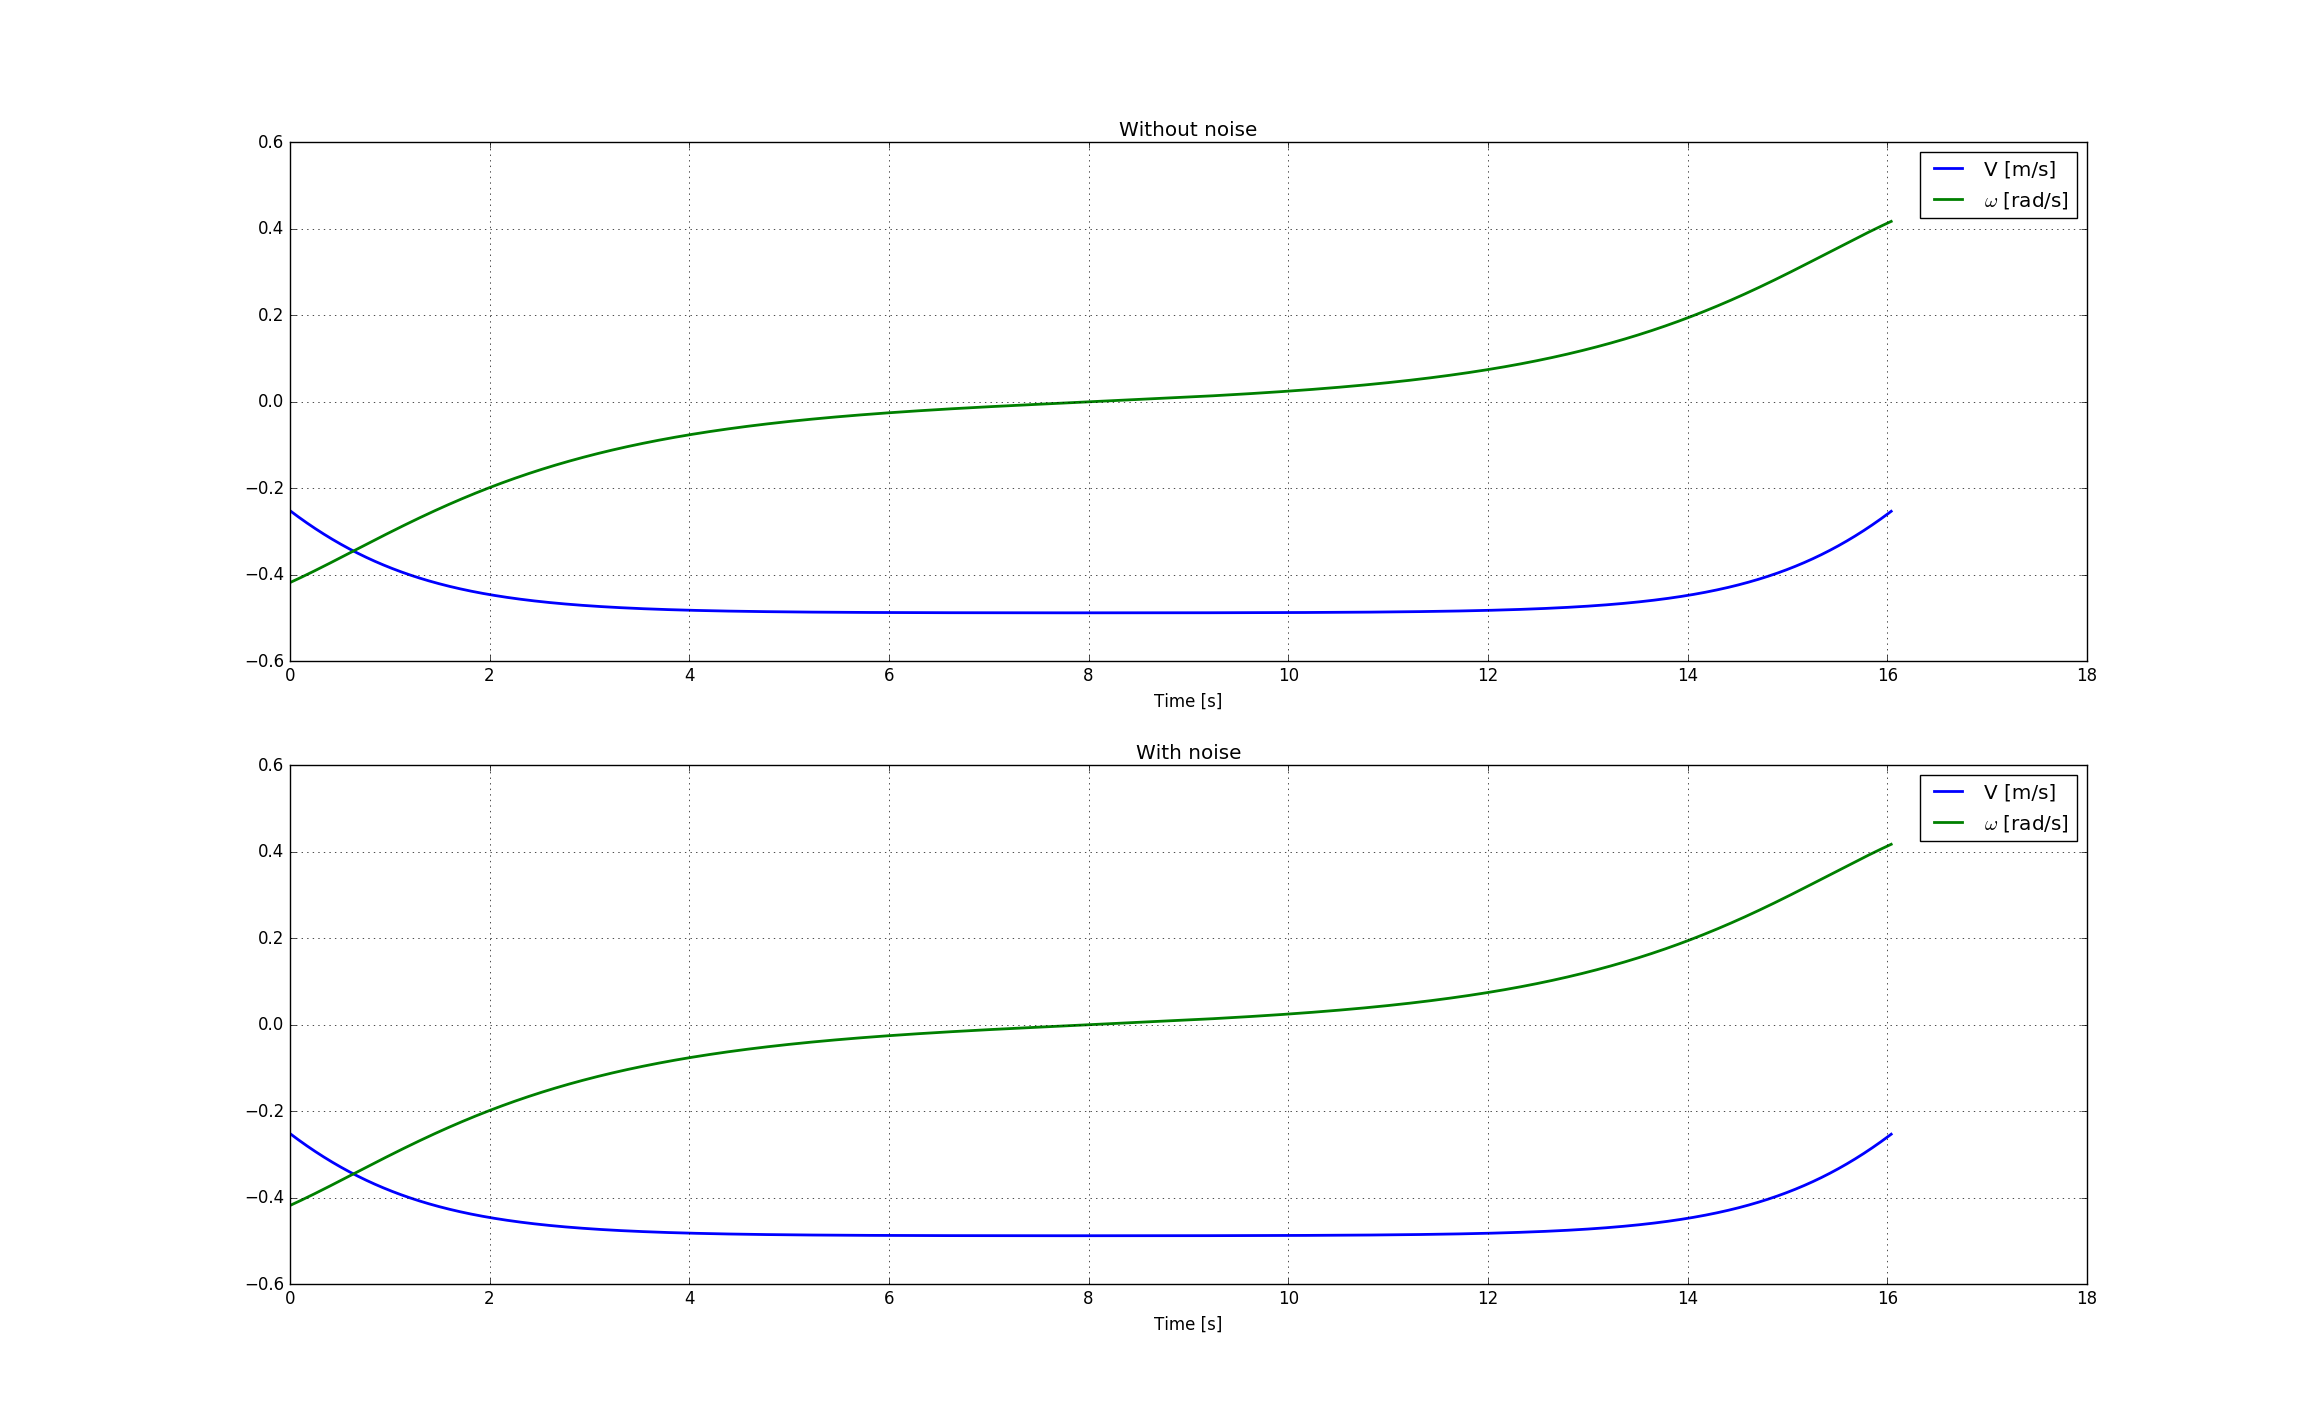
\includegraphics[width=\textwidth]{../Figures/hw1_1_v_ctrl.png}
	\end{figure}
\end{enumerate}

\section{Differential Flatness}
\begin{enumerate}
	\item Let $\psi_1(t) = 1, \psi_2(t) = t, \psi_3(t) = t^2$, and $\psi_4(t) = t^3$, then $n = 4$ and
	\begin{align*}
		x(t) &= \sum_{i=1}^n x_i\psi_i(t) = x_1 + x_2t + x_3t^2 + x_4t^3 \\
		y(t) &= \sum_{i=1}^n y_i\psi_i(t) = y_1 + y_2t + y_3t^2 + y_4t^3 \\
		\dot x(t) &= \sum_{i=1}^n x_i\dot \psi_i(t) = x_2 + 2x_3t + 3x_4t^2 \\
		\dot y(t) &= \sum_{i=1}^n y_i\dot \psi_i(t) = y_2 + 2y_3t + 3y_4t^2
	\end{align*}
	so the initial and final conditions can be expressed as
	\begin{align*}
		&x(0) = 0 = x_1 \\
		&y(0) = 0 = y_1 \\
		&x(t_f) = 5 = x_1 + x_2t_f + x_3t_f^2 + x_4t_f^3 \\
		&y(t_f) = 5 = y_1 + y_2t_f + y_3t_f^2 + y_4t_f^3 \\
		&\dot x(0) = V(0)\cos(\theta(0)) = 0.5\cos(-\pi/2) = 0 = x_2 \\
		&\dot y(0) = V(0)\sin(\theta(0)) = 0.5\sin(-\pi/2) = -0.5 = y_2 \\
		&\dot x(t_f) = V(t_f)\cos(\theta(t_f)) = 0.5\cos(-\pi/2) = 0 = x_2 + 2x_3t_f + 3x_4t_f^2 \\
		&\dot y(t_f) = V(t_f)\sin(\theta(t_f)) = 0.5\sin(-\pi/2) = -0.5 = y_2 + 2y_3t_f + 3y_4t_f^2
	\end{align*}
	or more succinctly in matrix form,
	\begin{align*}
		\left(\begin{array}{cccc}
		1 & 0 & 0 & 0 \\
		1 & t_f & t_f^2 & t_f^3 \\
		0 & 1 & 0 & 0 \\
		0 & 1 & 2t_f & 3t_f^2
		\end{array}\right)
		\left(\begin{array}{c}
		x_1 \\
		x_2 \\
		x_3 \\
		x_4
		\end{array}\right) =
		\left(\begin{array}{cccc}
		1 & 0 & 0 & 0 \\
		1 & 15 & 225 & 3375 \\
		0 & 1 & 0 & 0 \\
		0 & 1 & 30 & 675
		\end{array}\right)
		\left(\begin{array}{c}
			x_1 \\
			x_2 \\
			x_3 \\
			x_4
		\end{array}\right) &= 
		\left(\begin{array}{c}
			0 \\
			5 \\
			0 \\
			0
		\end{array}\right) =
		\left(\begin{array}{c}
		x(0) \\
		x(t_f) \\
		\dot x(0) \\
		\dot x(t_f)
		\end{array}\right) \\
		\left(\begin{array}{cccc}
		1 & 0 & 0 & 0 \\
		1 & t_f & t_f^2 & t_f^3 \\
		0 & 1 & 0 & 0 \\
		0 & 1 & 2t_f & 3t_f^2
		\end{array}\right)
		\left(\begin{array}{c}
		y_1 \\
		y_2 \\
		y_3 \\
		y_4
		\end{array}\right) =
		\left(\begin{array}{cccc}
		1 & 0 & 0 & 0 \\
		1 & 15 & 225 & 3375 \\
		0 & 1 & 0 & 0 \\
		0 & 1 & 30 & 675
		\end{array}\right)
		\left(\begin{array}{c}
		y_1 \\
		y_2 \\
		y_3 \\
		y_4
		\end{array}\right) &= 
		\left(\begin{array}{c}
		0 \\
		5 \\
		-0.5 \\
		-0.5
		\end{array}\right) =
		\left(\begin{array}{c}
		y(0) \\
		y(t_f) \\
		\dot y(0) \\
		\dot y(t_f)
		\end{array}\right)
	\end{align*}
	We cannot set $V(t_f) = 0$ because then $J$ would be singular at time $t_f$, and we could not recover the flat outputs from the virtual control inputs.
	\item See submitted code. After solving for $x_i,y_i$ for $i = 1,\ldots,n$, we can recover
	\[
		\left(\begin{array}{c}
		x(t) \\
		y(t) \\
		\dot x(t) \\
		\dot y(t) \\
		\ddot x(t) \\
		\ddot y(t)
		\end{array}\right) =
		\left(\begin{array}{cccc}
		x_1 & x_2 & x_3 & x_4 \\
		y_1 & y_2 & y_3 & y_4 \\
		x_2 & 2x_3 & 3x_4 & 0 \\
		y_2 & 2y_3 & 3y_4 & 0 \\
		2x_3 & 6x_4 & 0 & 0 \\
		2y_3 & 6y_4 & 0 & 0
		\end{array}\right)
		\left(\begin{array}{c}
		1 \\
		t \\
		t^2 \\
		t^3
		\end{array}\right)
	\]
	along with the alignment angle
	\[
		\frac{\dot y(t)}{\dot x(t)} = \frac{V\sin(\theta(t))}{V\cos(\theta(t))} = \tan(\theta(t)) \Rightarrow \theta(t) = \arctan\left(\frac{\dot y(t)}{\dot x(t)}\right).
	\]
	Since $V > 0$, we take the positive root of
	\[
		\dot x(t)^2 + \dot y(t)^2 = V^2\cos^2(\theta(t)) + V^2\sin^2(\theta(t)) = V^2 \Rightarrow V(t) = \sqrt{\dot x(t)^2 + \dot y(t)^2},
	\]
	then the matrix $J$ is invertible, so we can calculate
	\begin{align*}
		J^{-1} &= \left(\begin{array}{cc}
		\cos(\theta) & -V\sin(\theta) \\
		\sin(\theta) & V\cos(\theta)
		\end{array}\right)^{-1} = 
		\frac{1}{V}\left(\begin{array}{cc}
		V\cos(\theta) & V\sin(\theta) \\
		-\sin(\theta) & \cos(\theta)
		\end{array}\right) \\
		\left(\begin{array}{c}
		a \\
		\omega
		\end{array}\right) &=
		J^{-1}\left(\begin{array}{c}
		\ddot x(t) \\
		\ddot y(t)
		\end{array}\right) =
		\left(\begin{array}{c}
		\ddot x(t)\cos(\theta) + \ddot y(t)\sin(\theta) \\
		\frac{1}{V}(-\ddot x(t)\sin(\theta) + \ddot y(t)\cos(\theta))
		\end{array}\right).
	\end{align*}
	Putting this all together, our state-trajectory is
	\begin{align*}
		x(t) &= x_1 + x_2t + x_3t^2 + x_4t^3 \\
		y(t) &= y_1 + y_2t + y_3t^2 + y_4t^3 \\
		\theta(t) &= \arctan\left(\frac{y_2 + 2y_3t + 3y_4t^2}{x_2 + 2x_3t + 3x_4t^2}\right)
	\end{align*}
	and our control history is
	\begin{align*}
		V(t) &= \sqrt{(x_2 + 2x_3t + 3x_4t^2)^2 + (y_2 + 2y_3t + 3y_4t^2)^2} \\
		\omega(t) &= \frac{1}{V(t)}\left(-(2x_3 + 6x_4t)\sin(\theta(t)) + (2y_3 + 6y_4t)\cos(\theta(t))\right)
	\end{align*}
	\item See submitted code. Given $\dot s(t) = V(t)$ with $s(0) = 0$, we can integrate to get the path parameter
	\[
		s(t) = \int_0^t V(t')dt' - V(0)
	\]
	We wish to find an alternative velocity control $\tilde V(s)$ that satisfies the control saturation constraints. Then, the corresponding angular velocity control and time history are
	\[
		\tilde \omega(s) = \omega(s) \frac{\tilde V(s)}{V(s)}, \quad
		\tau(s) = \int_0^s \frac{ds'}{\tilde V(s')}.
	\]
	Combining the constraint $|\tilde V(s)| \leq 0.5$ m/s with
	\[
		|\tilde \omega(s)| = \left|\omega(s) \frac{\tilde V(s)}{V(s)}\right| \leq 1 \mbox{ rad/s} \Rightarrow |\tilde V(s)| \leq \frac{V(s)}{|\omega(s)|} \mbox{ for } \omega(s) \neq 0
	\]
	we see that a viable choice is
	\[
		\tilde V(s) = \begin{cases}
			\min(V(s), 0.5) & \mbox{ if } \omega(s) = 0 \\
			\min\left(V(s), \frac{V(s)}{|\omega(s)|}, 0.5\right) & \mbox{ if } \omega(s) \neq 0
		\end{cases}
	\]
	\item See submitted code.
		\begin{figure}[H]
			\centering
			\title{\bf Trajectory $(x(t), y(t))$}
			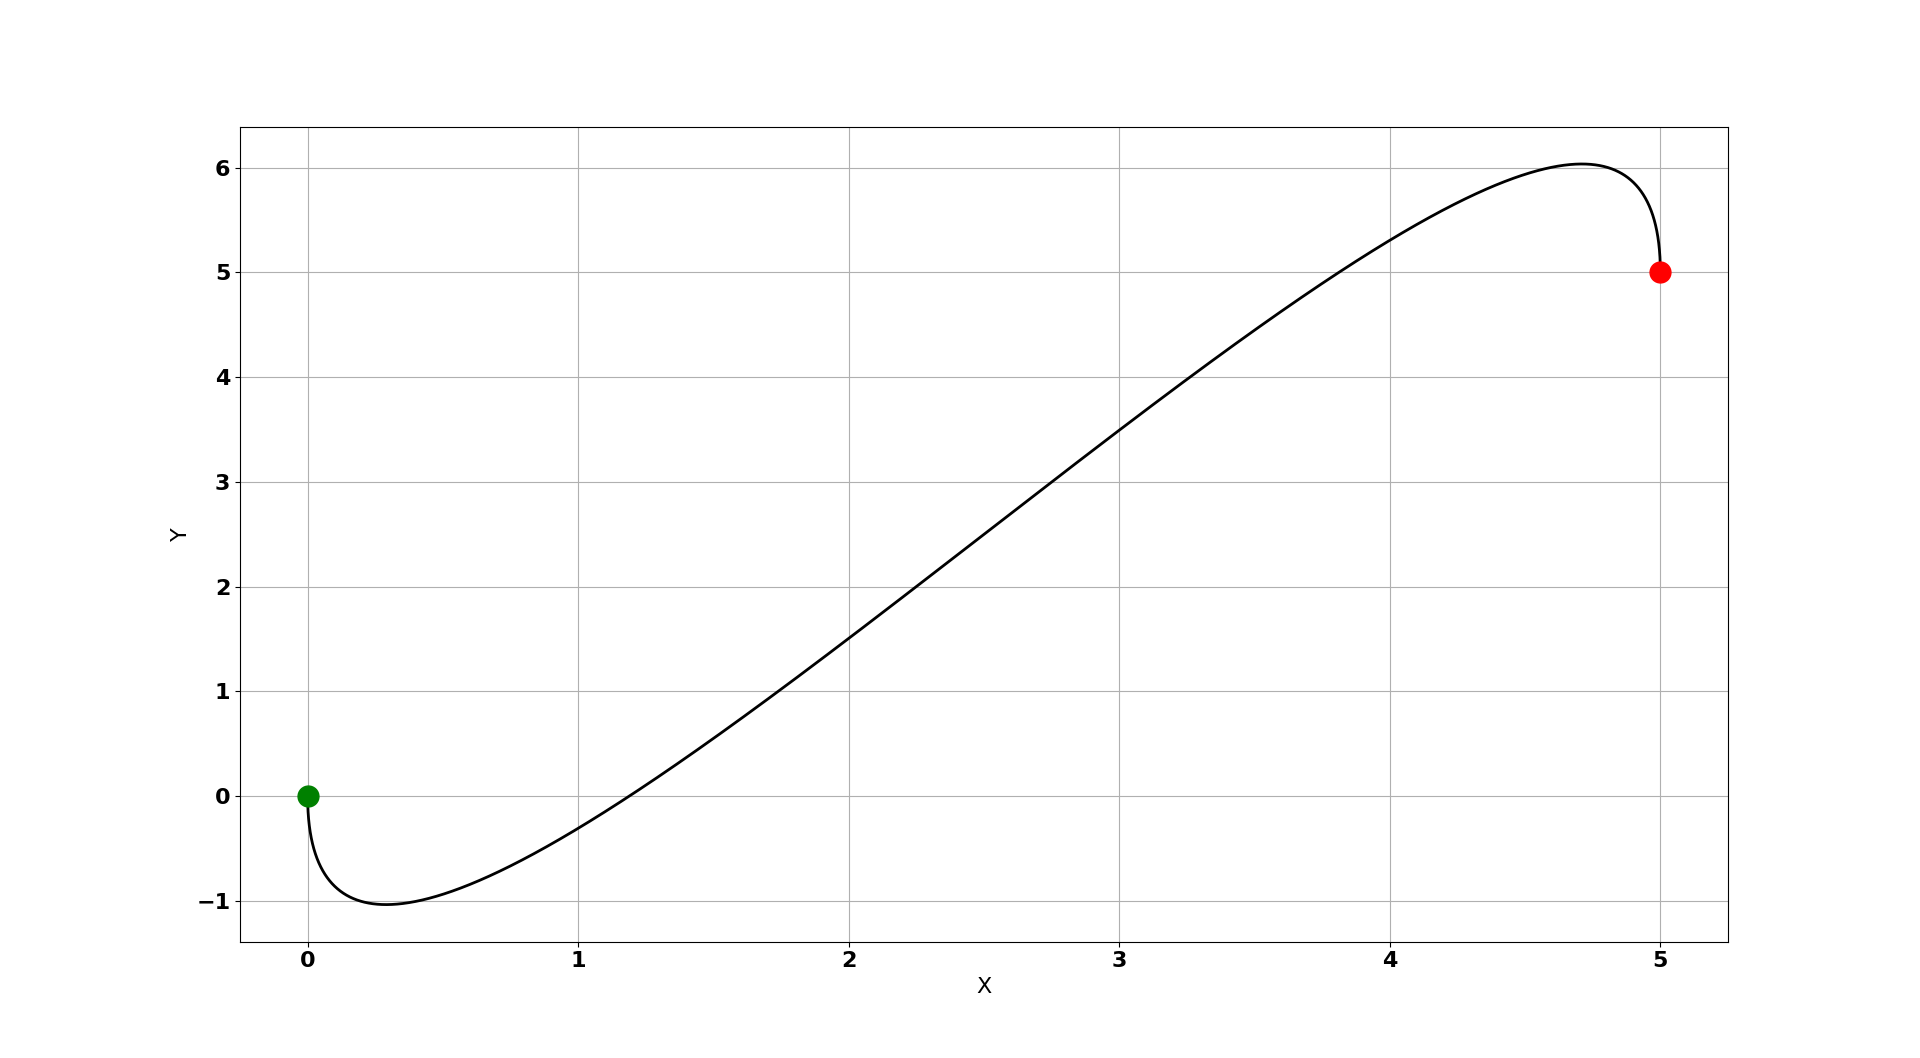
\includegraphics[width=\textwidth]{../Figures/hw1_2_iv_a.png}
		\end{figure}
		\begin{figure}[H]
			\centering
			\title{\bf Arc-length $s(t)$}
			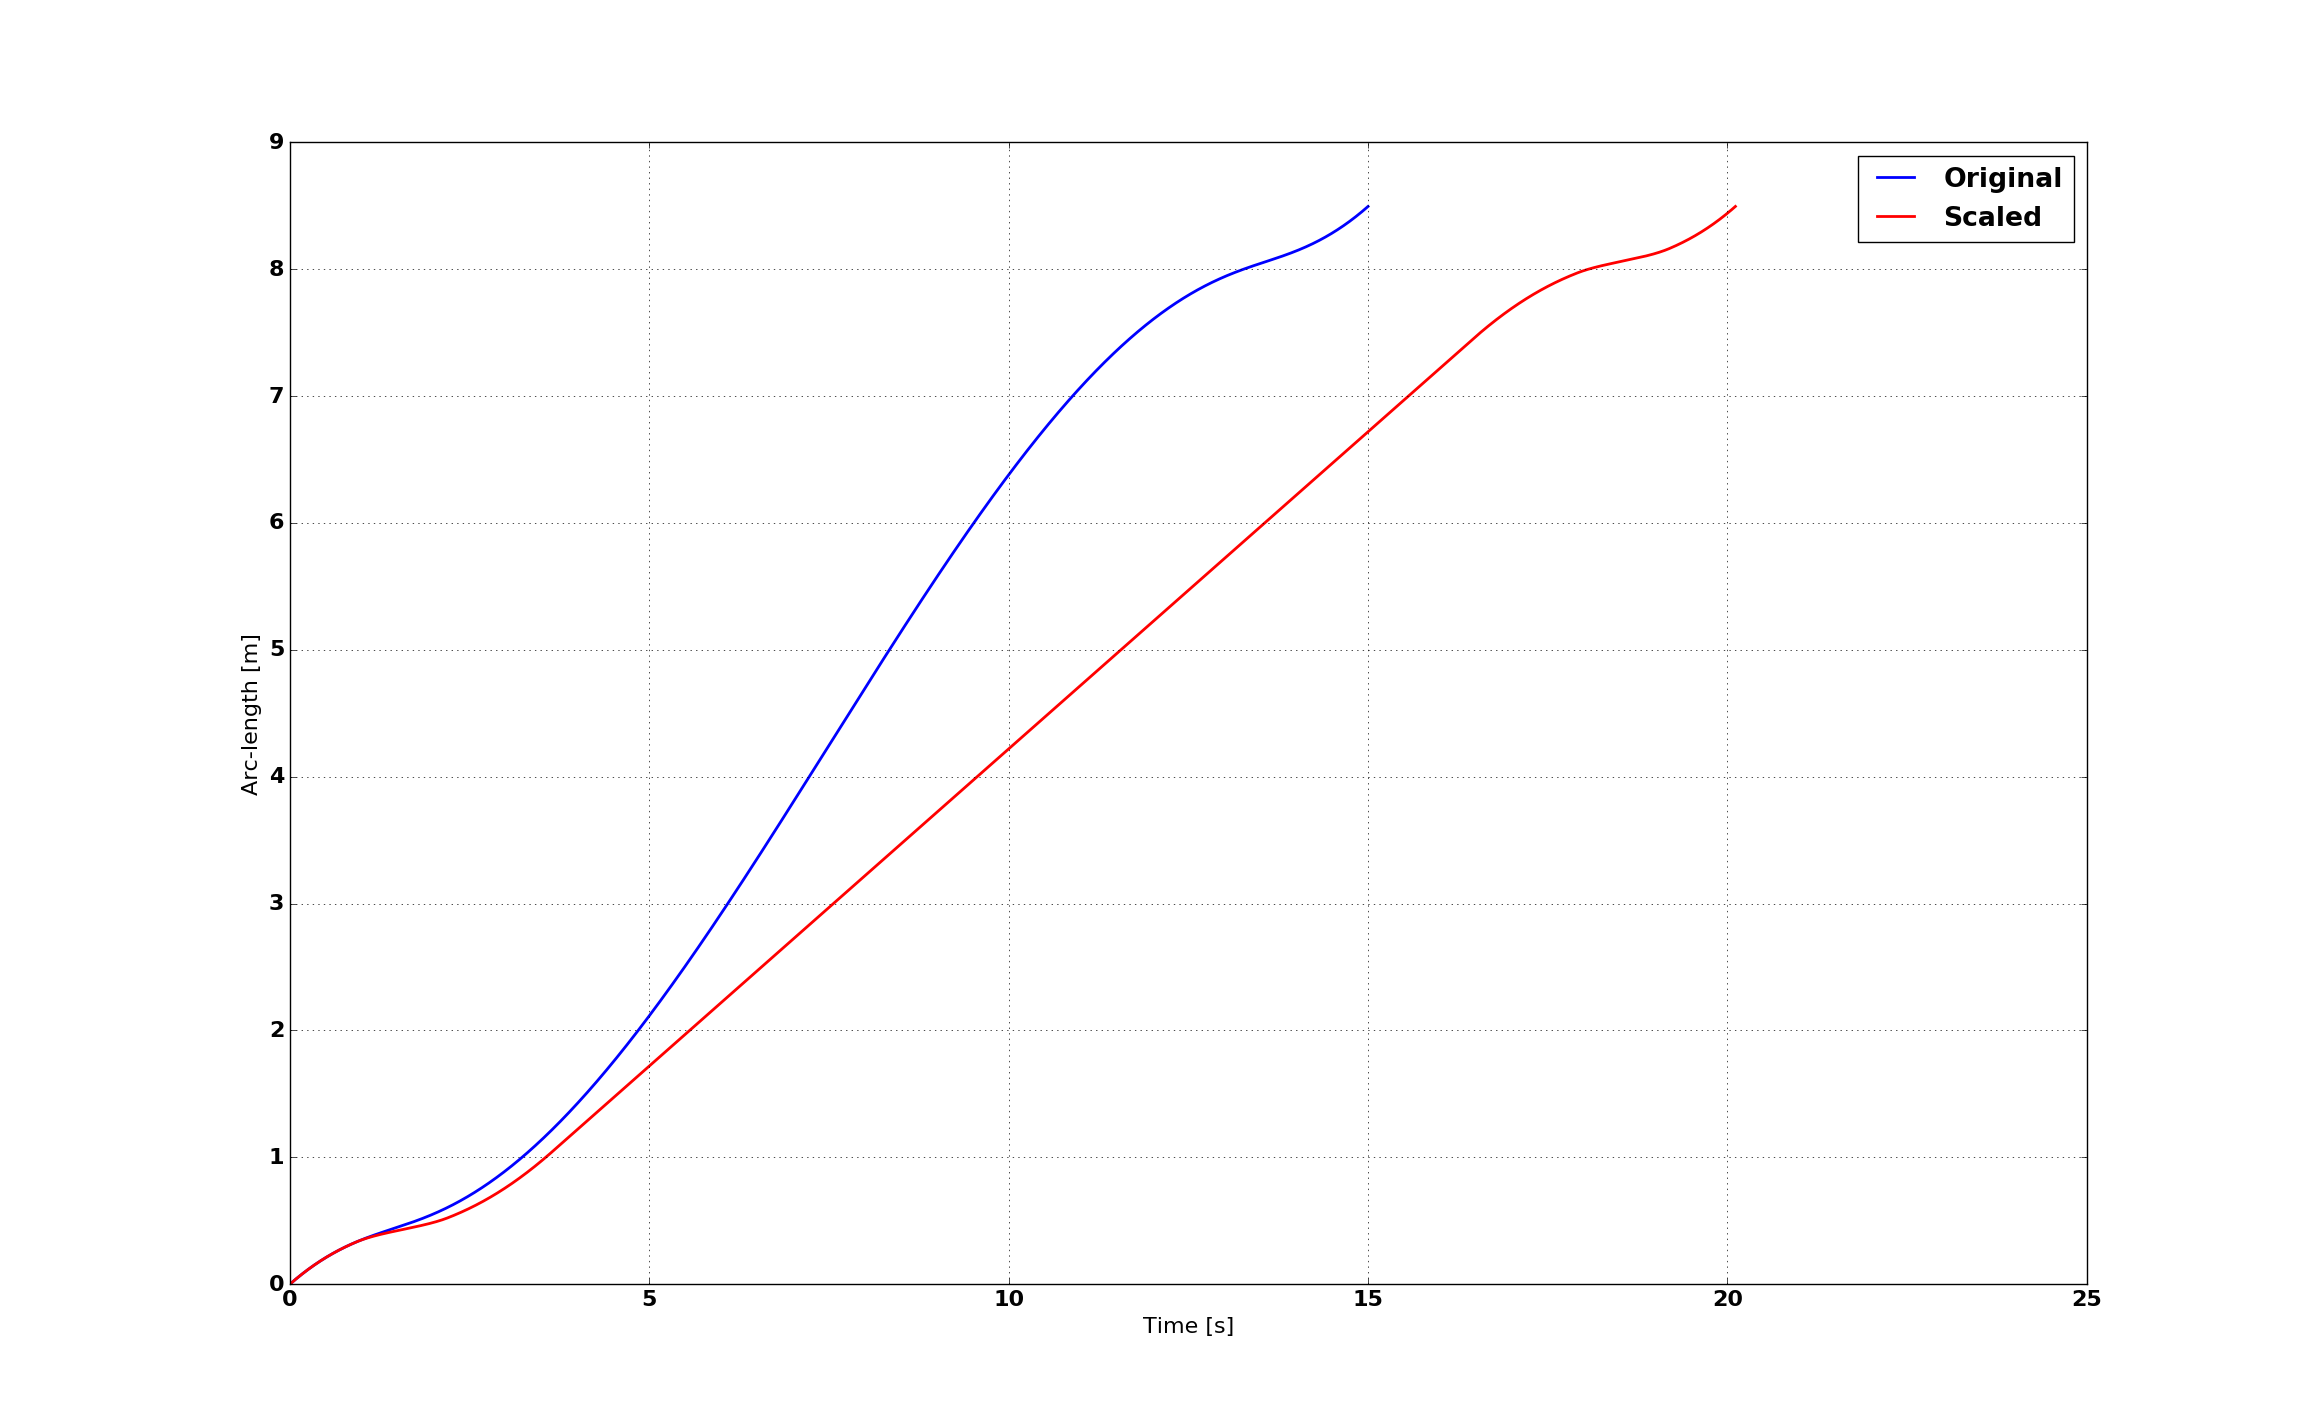
\includegraphics[width=\textwidth]{../Figures/hw1_2_iv_b.png}
		\end{figure}
		\begin{figure}[H]
			\centering
			\title{\bf History of $V$ and $\omega$}
			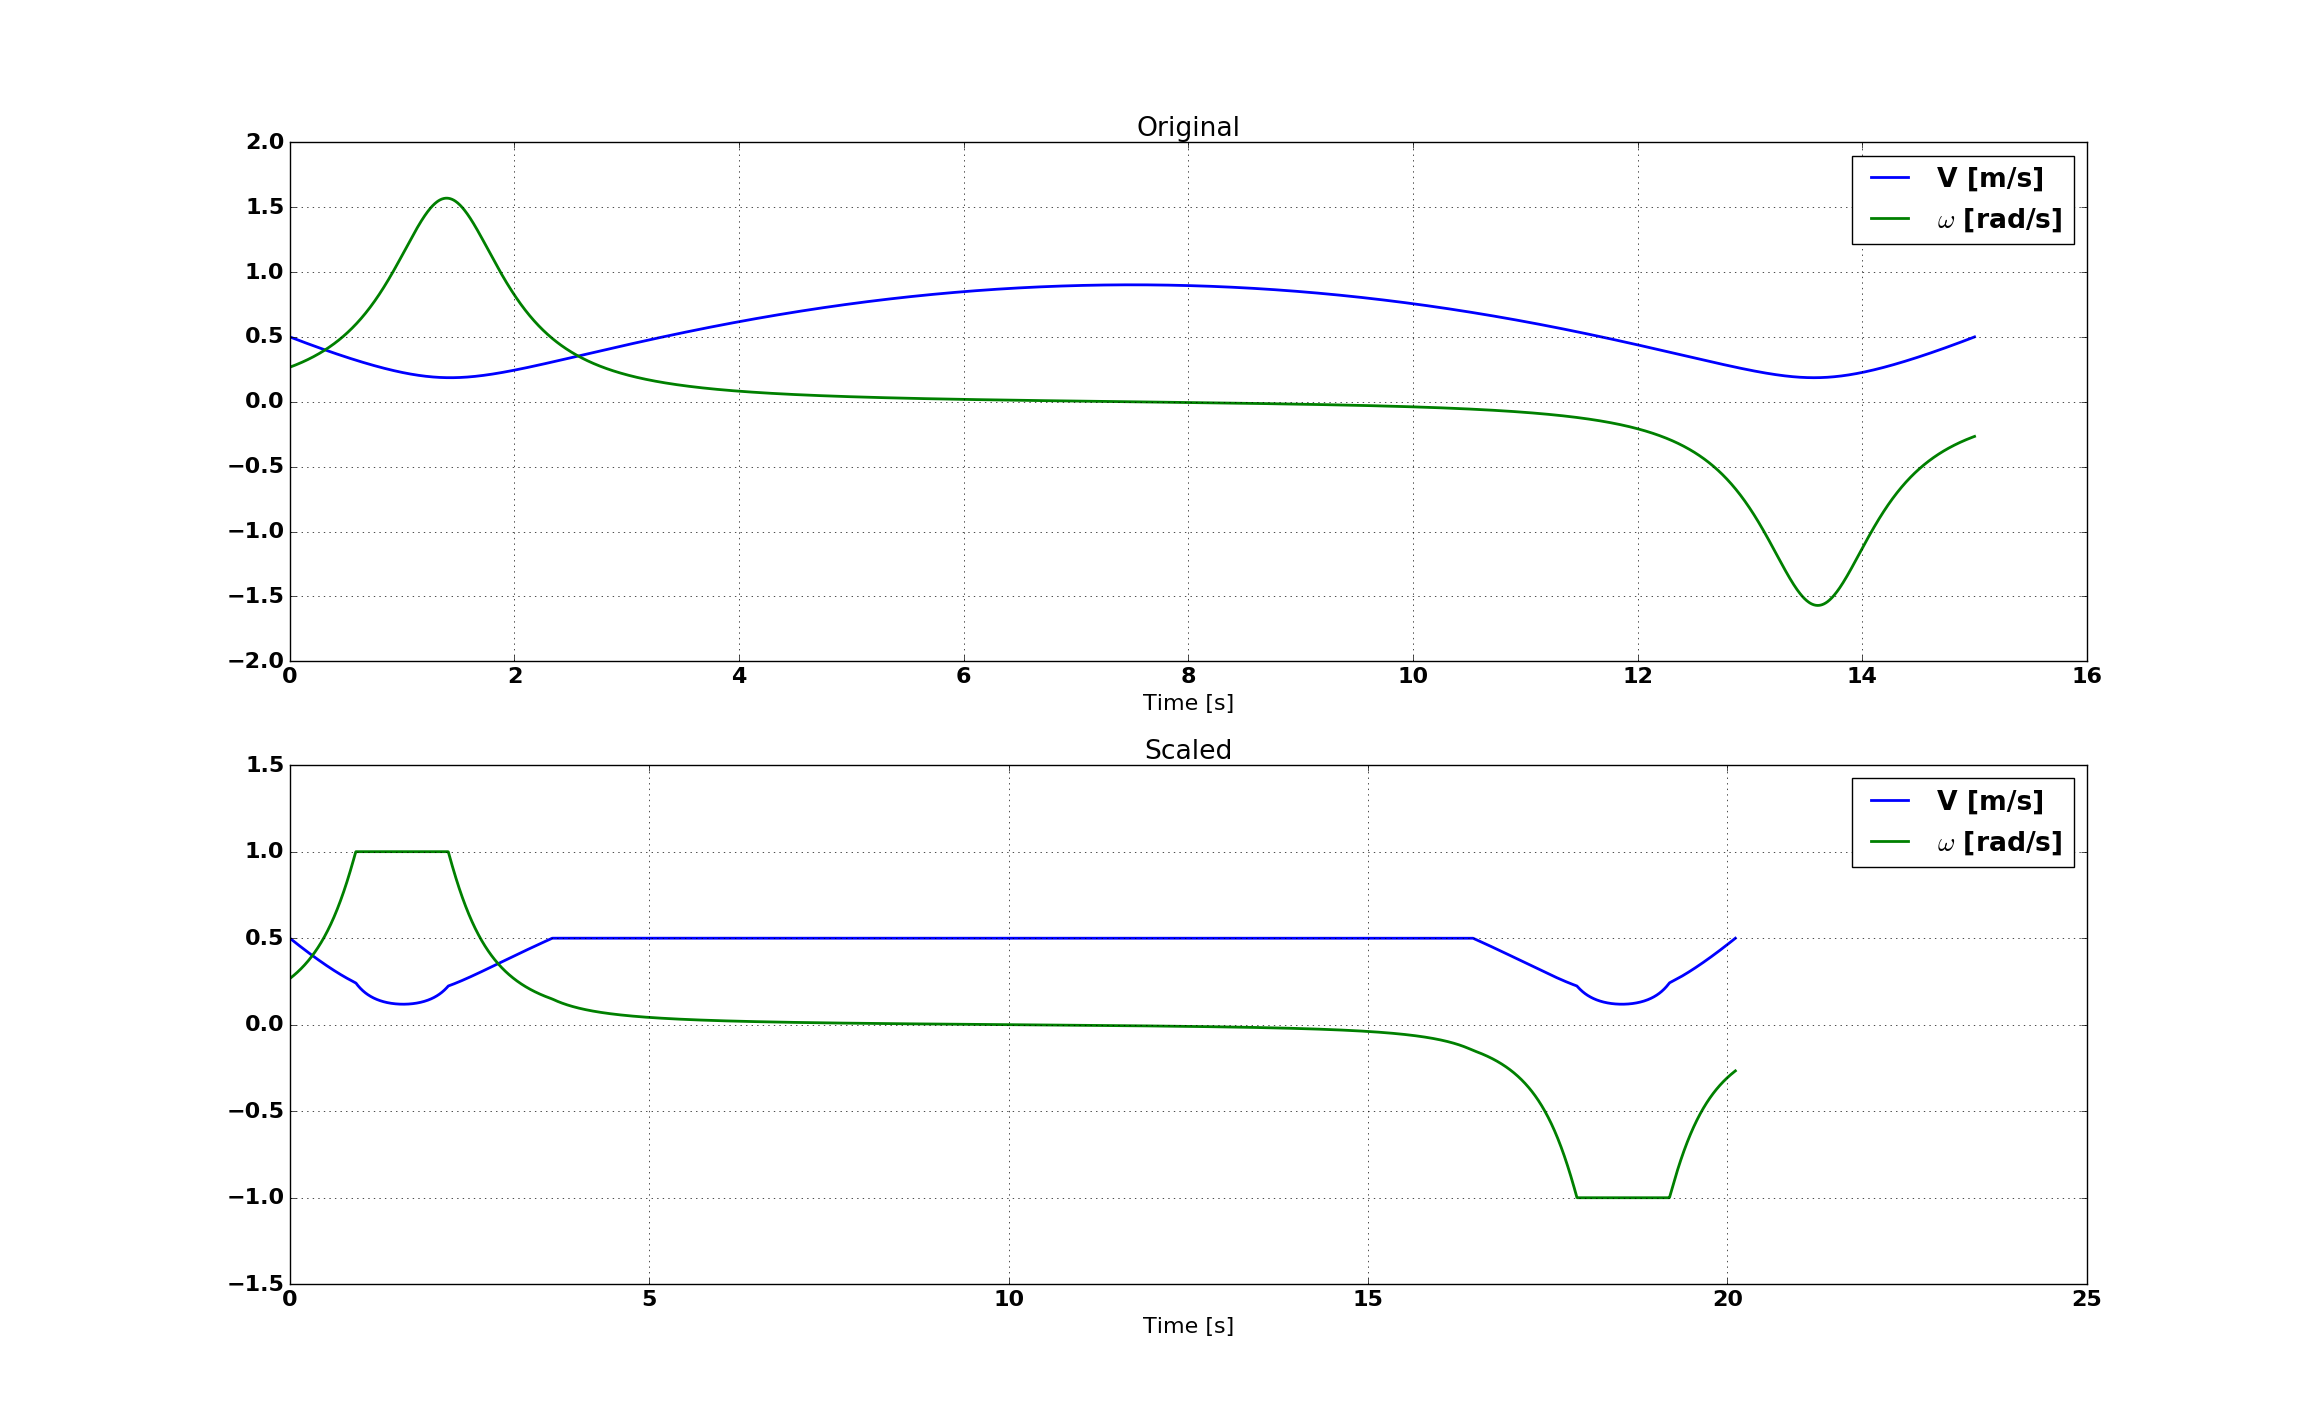
\includegraphics[width=\textwidth]{../Figures/hw1_2_iv_c.png}
		\end{figure}
	\item See submitted code.
	\begin{figure}[H]
		\centering
		\title{\bf Trajectory $(x(t), y(t))$}
		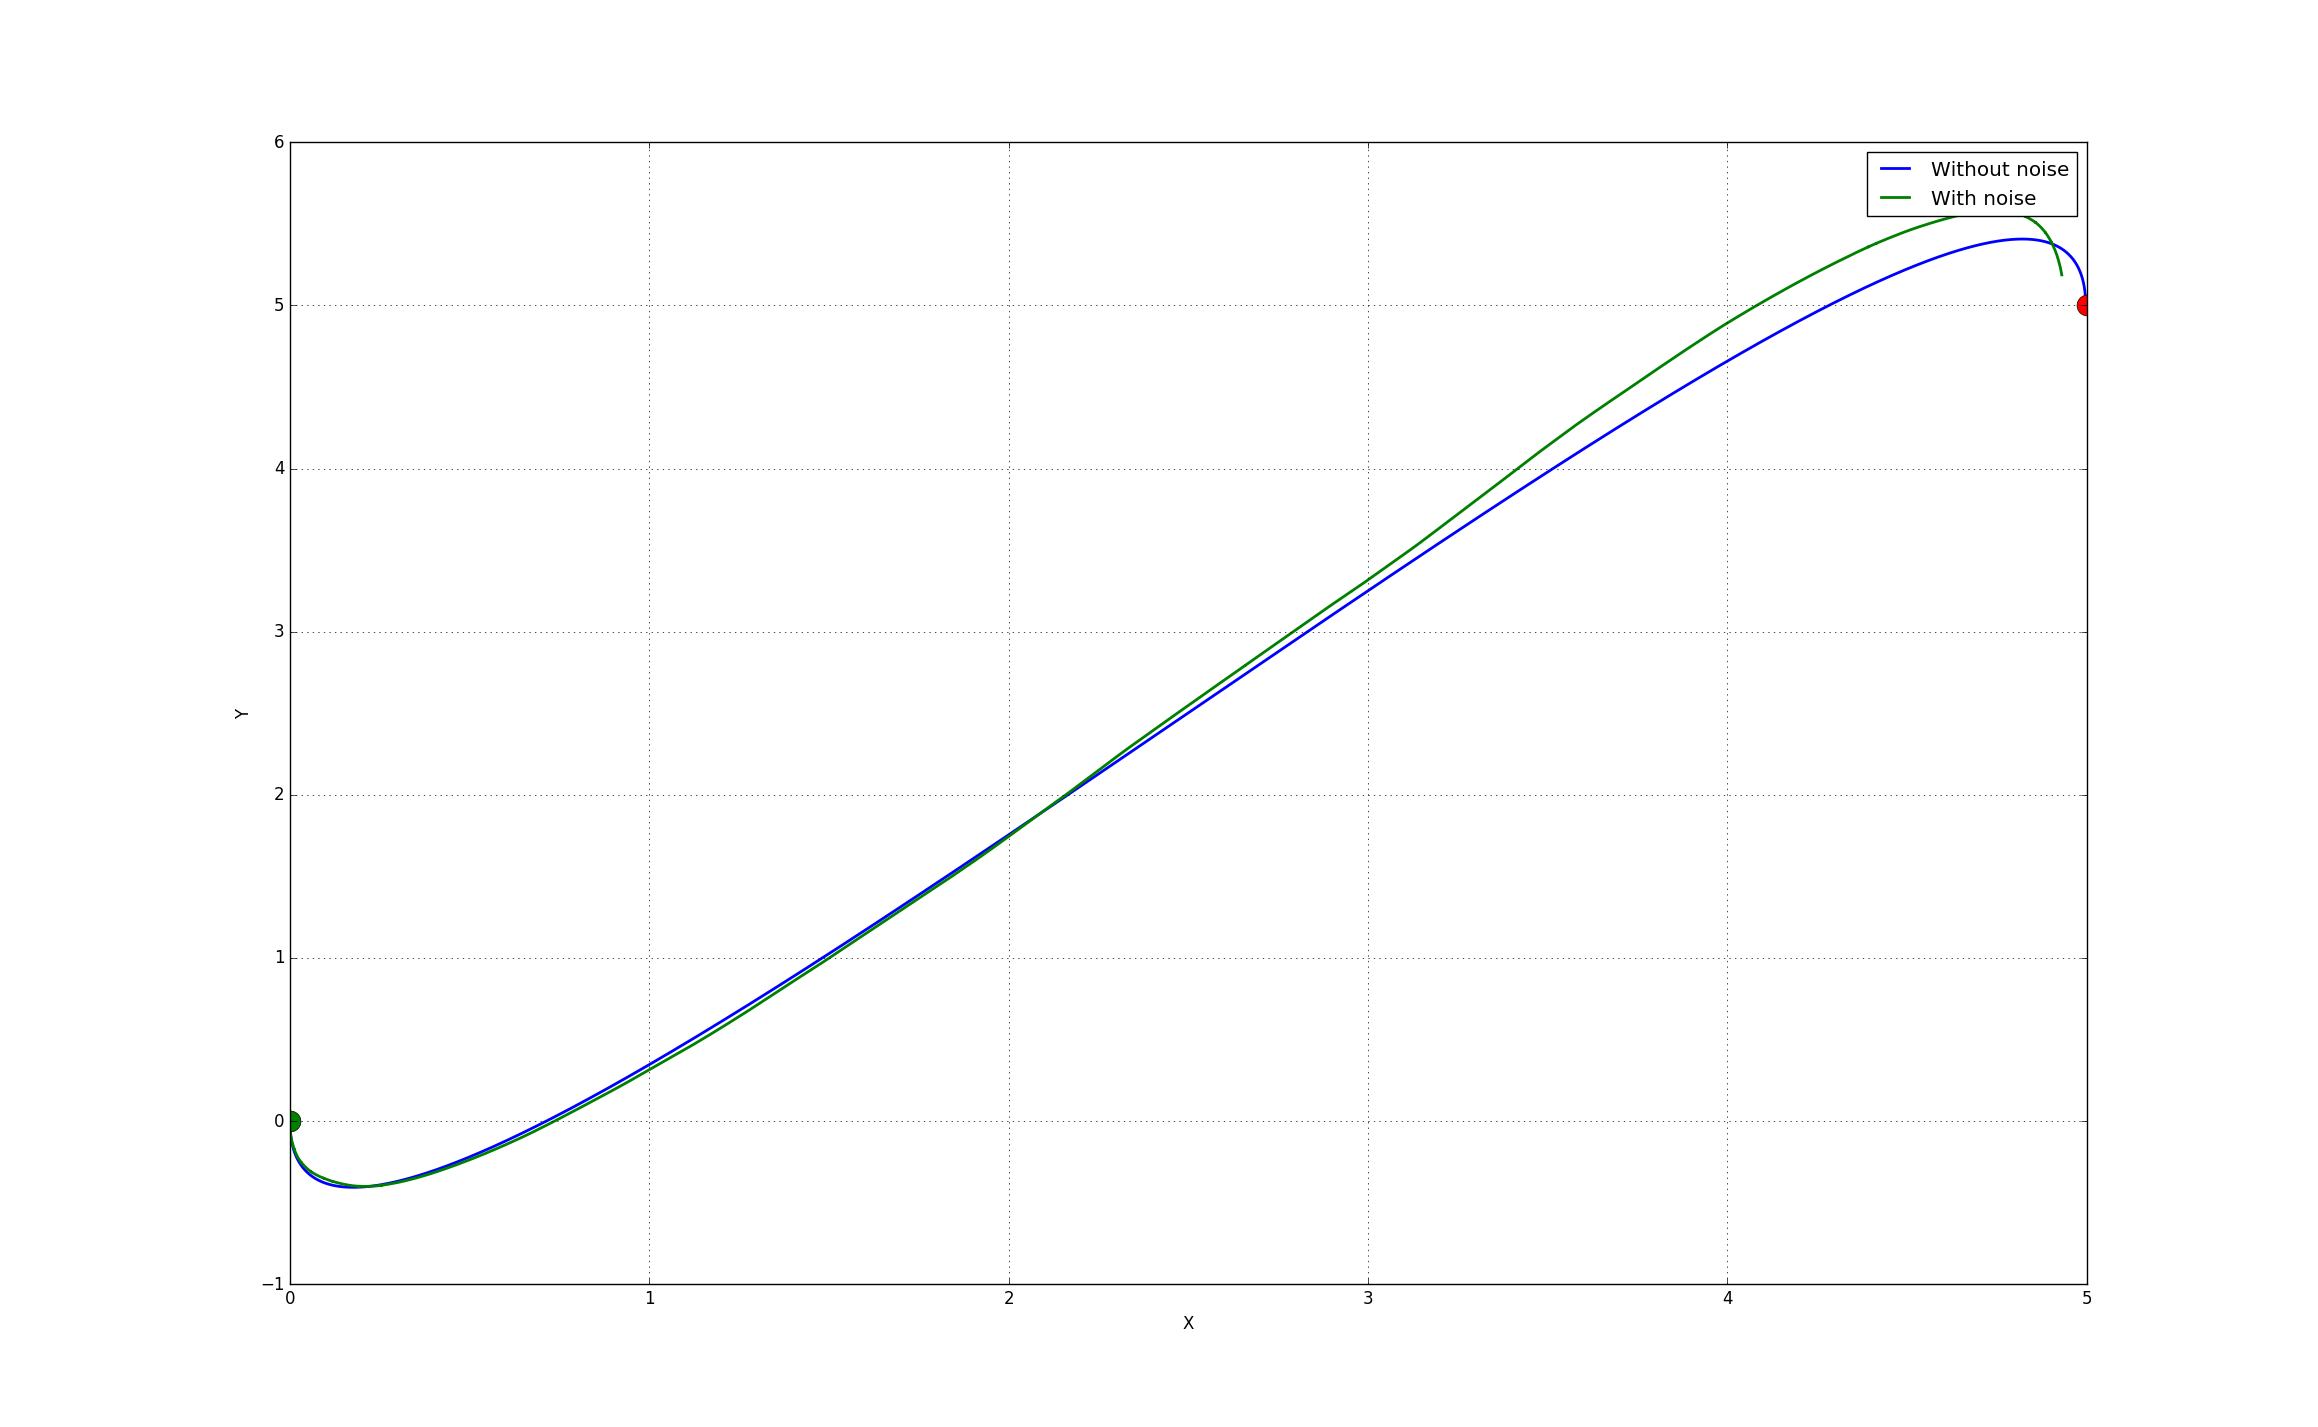
\includegraphics[width=\textwidth]{../Figures/hw1_2_v_traj.png}
	\end{figure}
	\begin{figure}[H]
		\centering
		\title{\bf History of $V$ and $\omega$}
		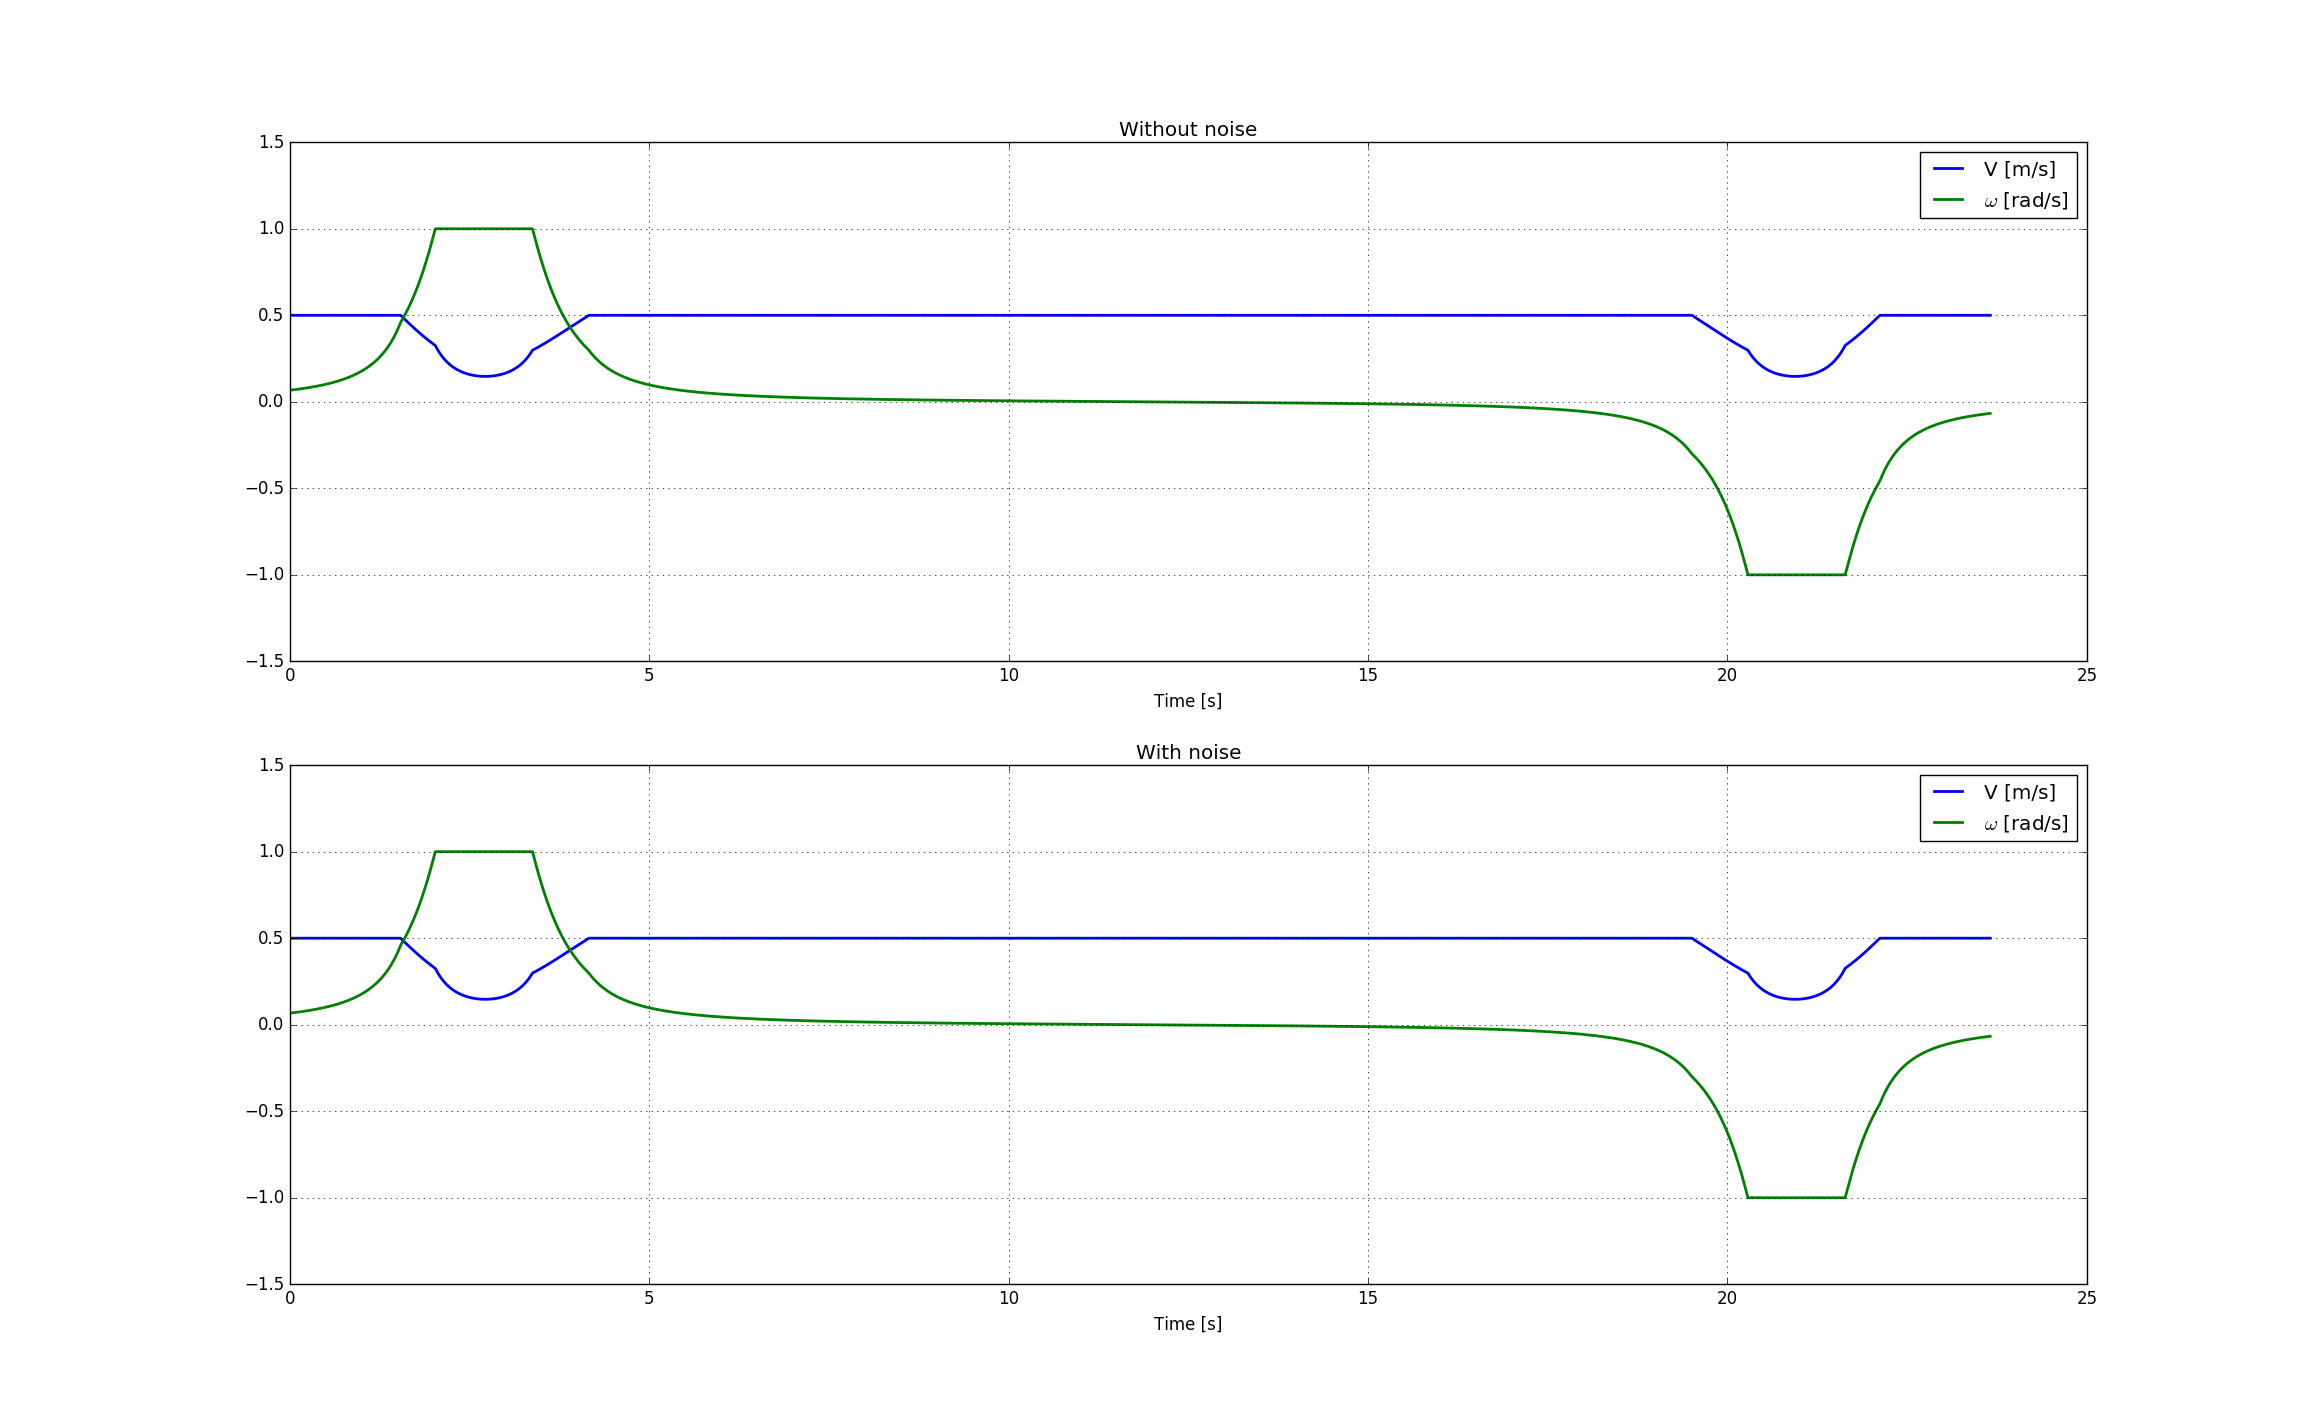
\includegraphics[width=\textwidth]{../Figures/hw1_2_v_ctrl.png}
	\end{figure}
\end{enumerate}

\section{Closed-loop Control I}
\begin{enumerate}
	\item See submitted code. We are given the control law
	\begin{align*}
		V &= k_1\rho\cos(\alpha) \\
		\omega &= k_2\alpha + k_1\frac{\sin(\alpha)\cos(\alpha)}{\alpha}(\alpha + k_3\delta)
	\end{align*}
	for the ODE system
	\begin{align*}
		\dot \rho(t) &= -V(t)\cos(\alpha(t)) \\
		\dot \alpha(t) &= V(t)\frac{\sin(\alpha(t))}{\rho(t)} - \omega(t) \\
		\dot \delta(t) &= V(t)\frac{\sin(\alpha(t))}{\rho(t)}
	\end{align*}
	where $k_1,k_2,k_3 > 0$ are constants. From Homework 1, Figure 2, we readily see that for a starting position $(x,y,\theta)$ and final position $(x_g,y_g,\theta_g)$, the incremental change in polar coordinates is
	\begin{align*}
		\rho &= \sqrt{(x_g - x)^2 + (y_g - y)^2} \\
		\tan(\alpha + \theta) = \frac{y_g - y}{x_g - x} \Rightarrow \alpha &= \arctan{\left(\frac{y_g - y}{x_g - x}\right)} - \theta \\
		\alpha + \theta = \delta + \theta_g \Rightarrow \delta &= \alpha + \theta - \theta_g
	\end{align*}
	\item See submitted code. The parameters used were
	\begin{align*}
		(x_0,y_0,\theta_0,t_f) &=
		\begin{cases}
			(5,10,-\pi/2,20) & \mbox{for forward parking} \\
			(5,0,-\pi/2,12) & \mbox{for reverse parking} \\
			(0,5,-\pi/2,18) & \mbox{for parallel parking}
		\end{cases} \\
		(k_1,k_2,k_3) &=
		\begin{cases}
			(0.5,0.5,1.2) & \mbox{for forward parking} \\
			(1.45,0.01,1.45) & \mbox{for reverse parking} \\
			(0.5,0.5,1.2) & \mbox{for parallel parking}
		\end{cases}
	\end{align*}
	\begin{figure}[H]
		\centering
		\title{\bf Forward Trajectory}
		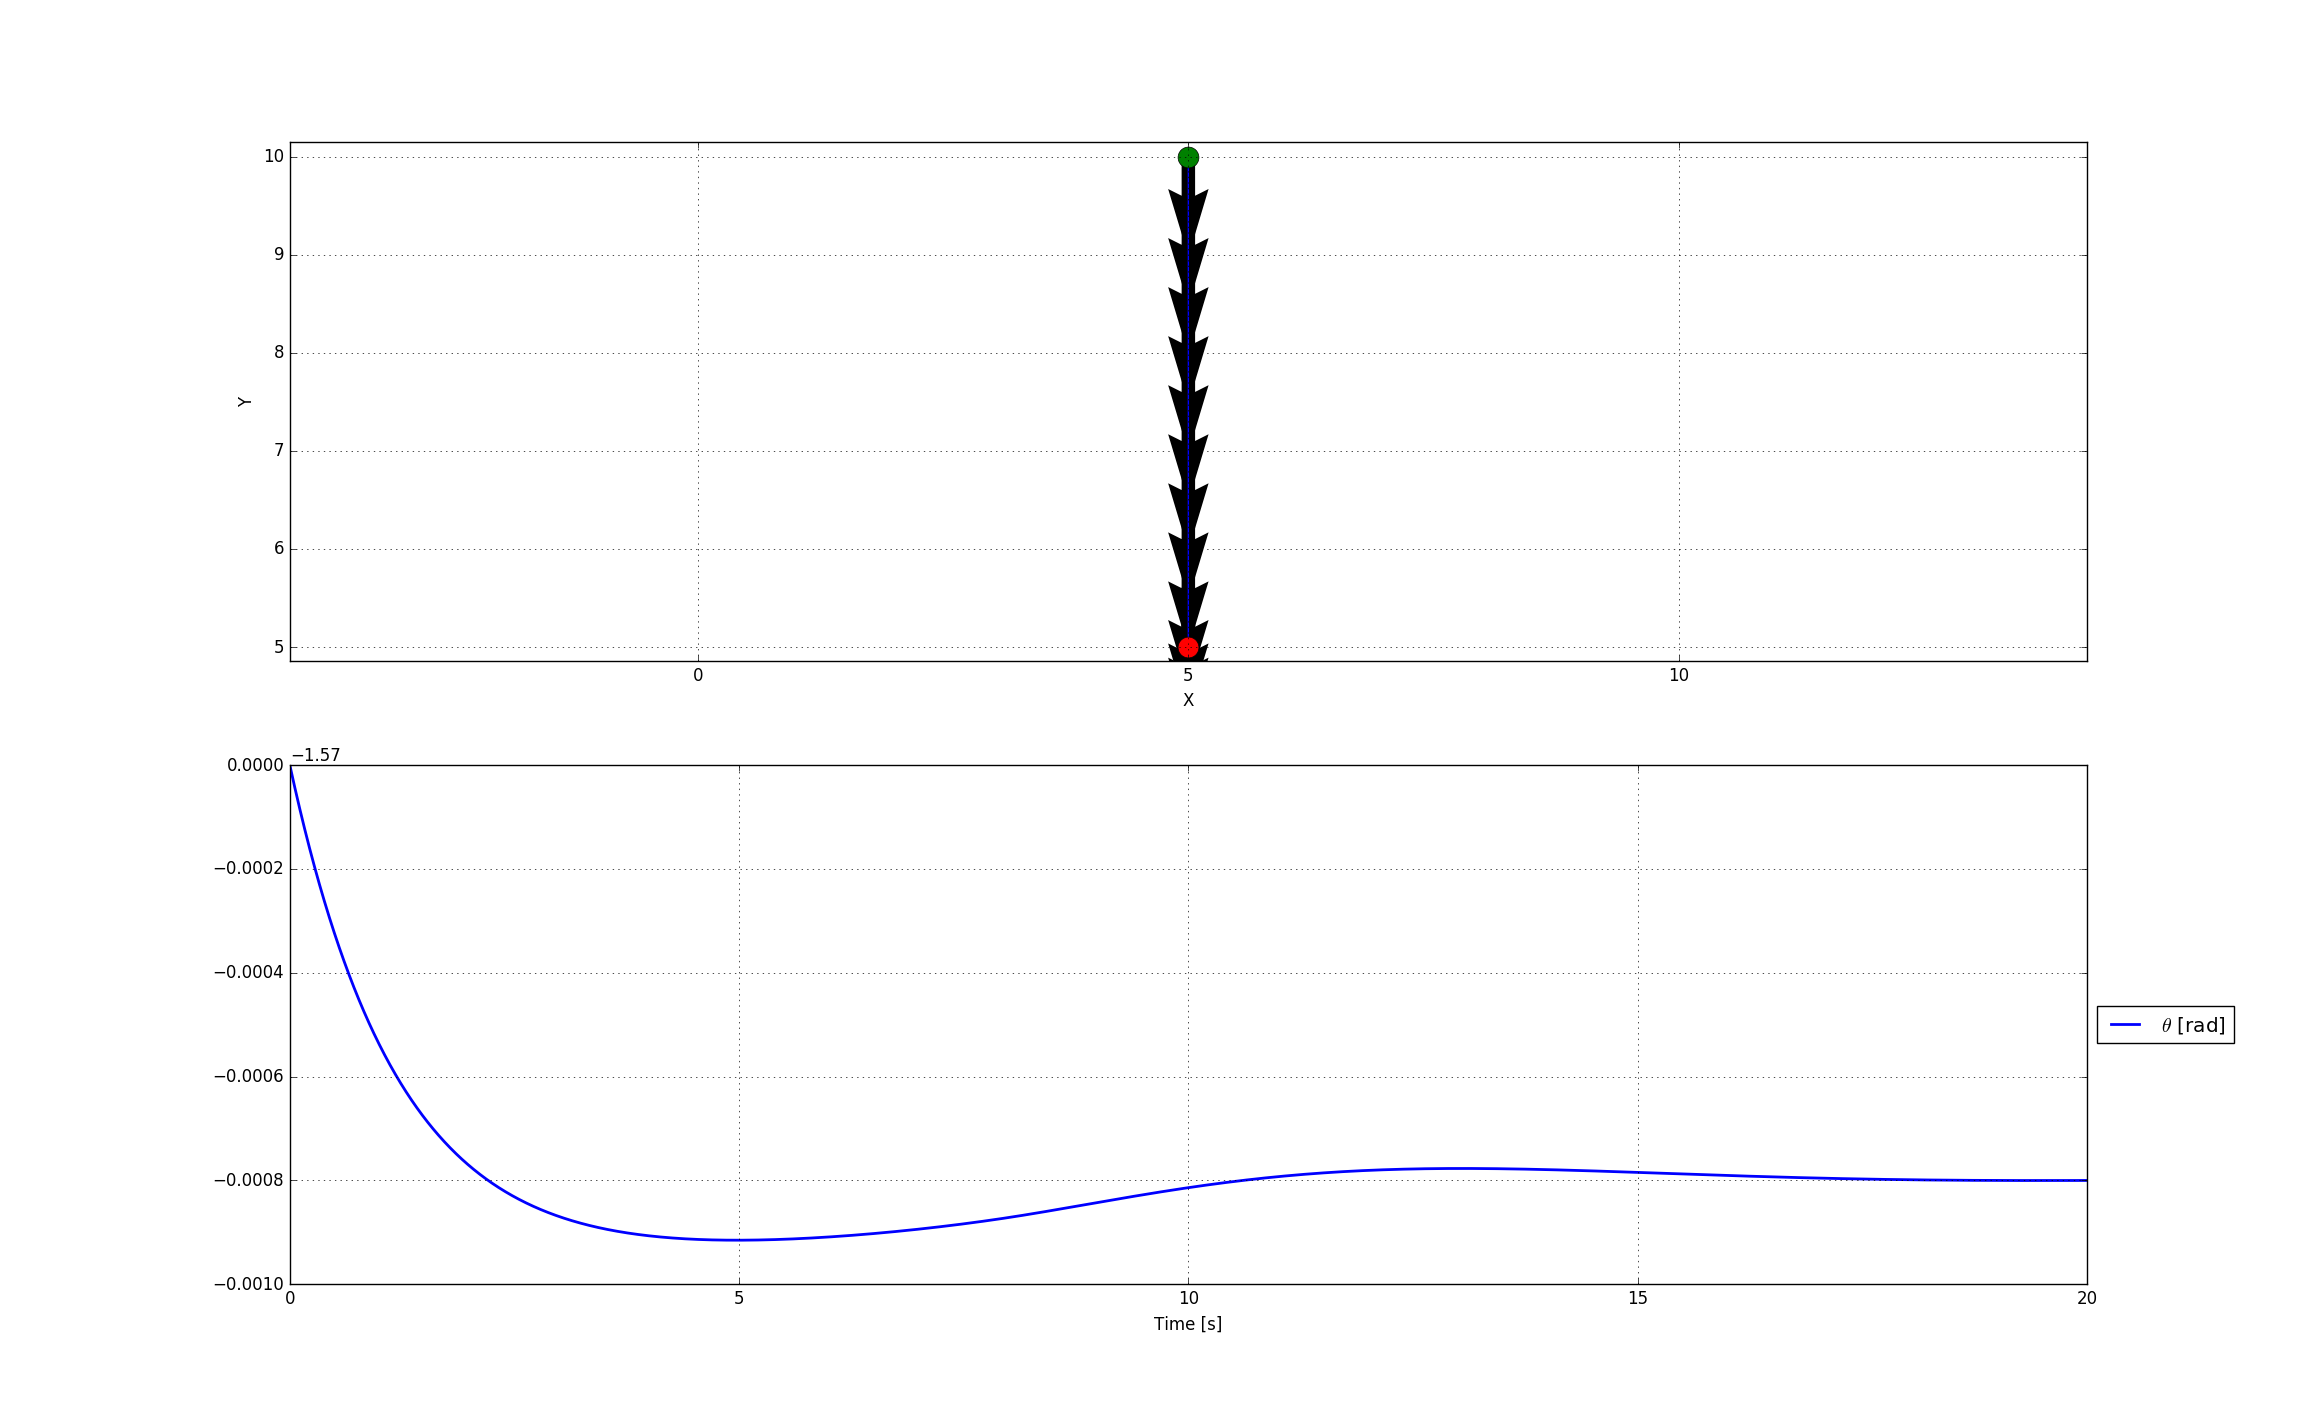
\includegraphics[width=\textwidth]{../Figures/hw1_3_ii_a_forward.png}
	\end{figure}
	\begin{figure}[H]
		\centering
		\title{\bf Forward Control}
		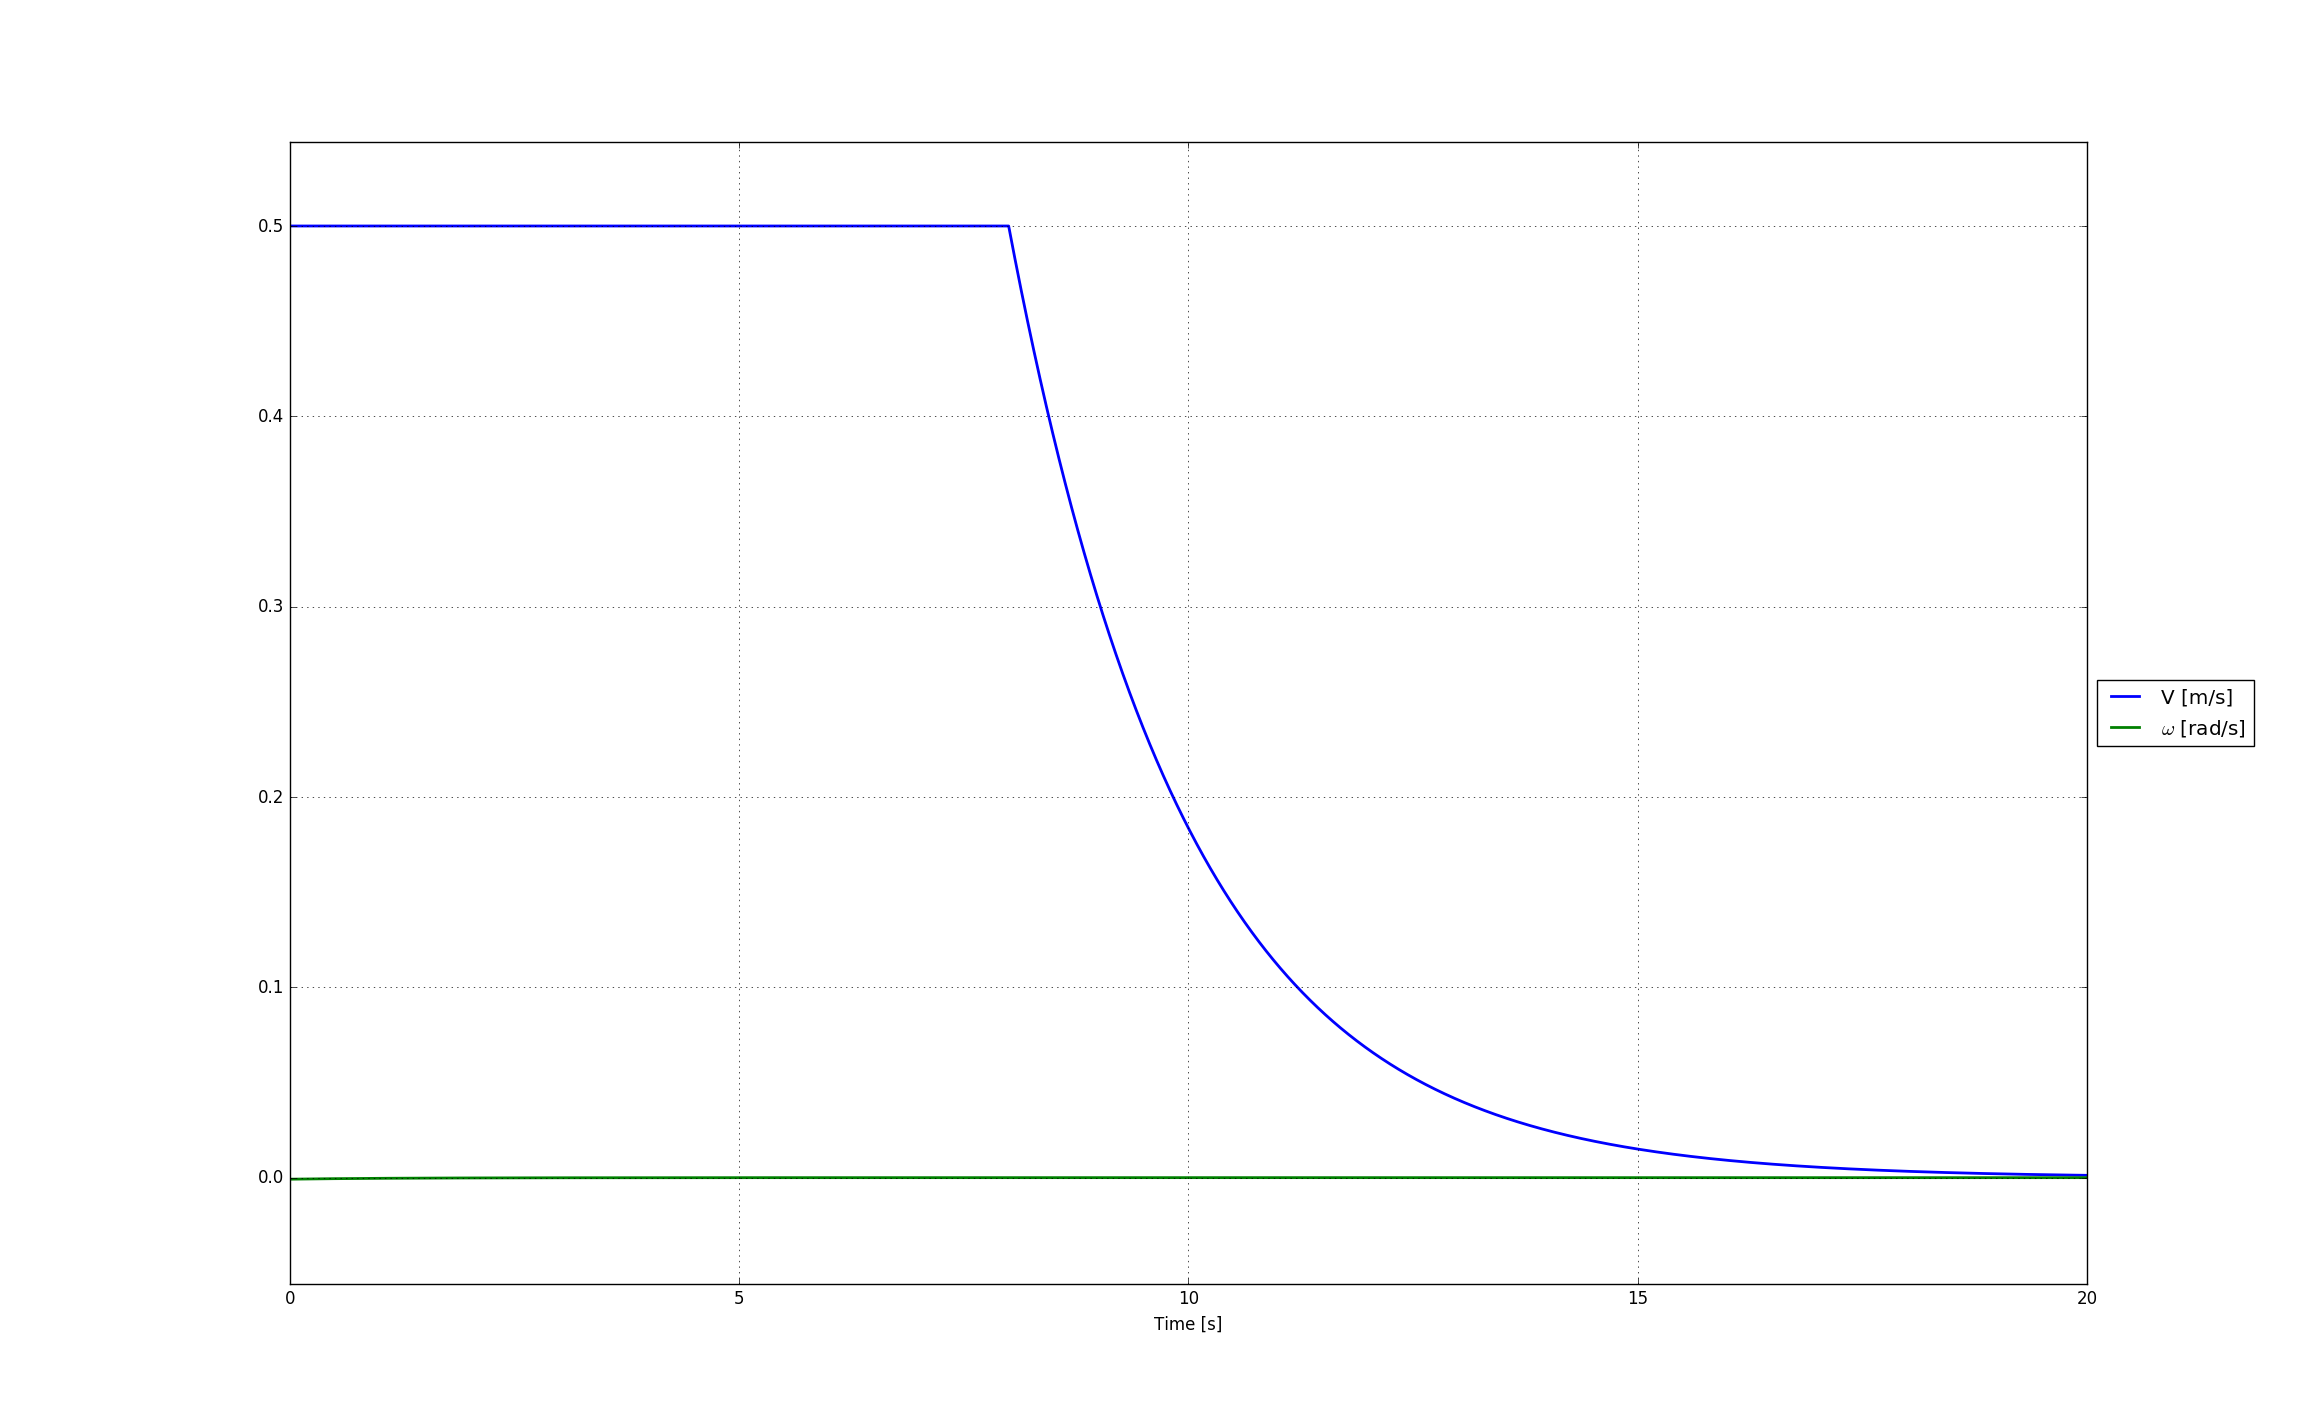
\includegraphics[width=\textwidth]{../Figures/hw1_3_ii_b_forward.png}
	\end{figure}
	\begin{figure}[H]
		\centering
		\title{\bf Reverse Trajectory}
		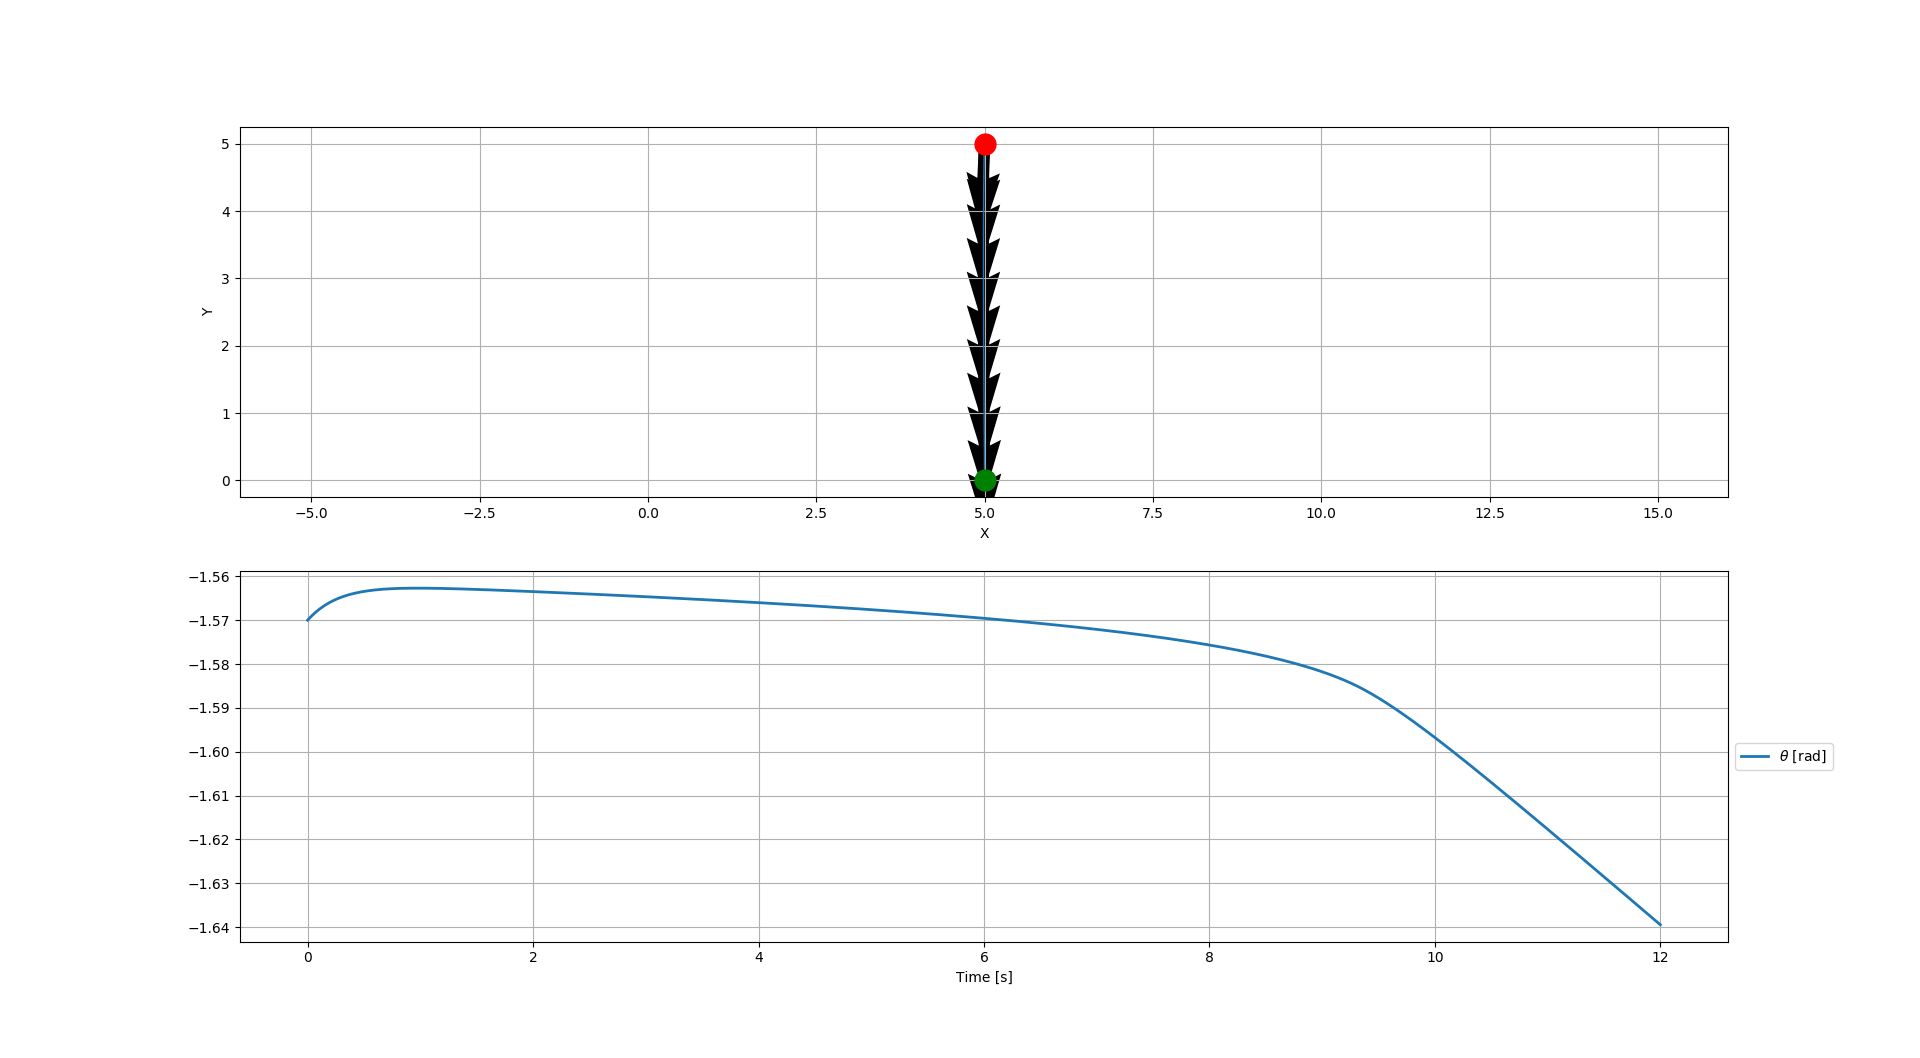
\includegraphics[width=\textwidth]{../Figures/hw1_3_ii_a_reverse.png}
	\end{figure}
	\begin{figure}[H]
		\centering
		\title{\bf Reverse Control}
		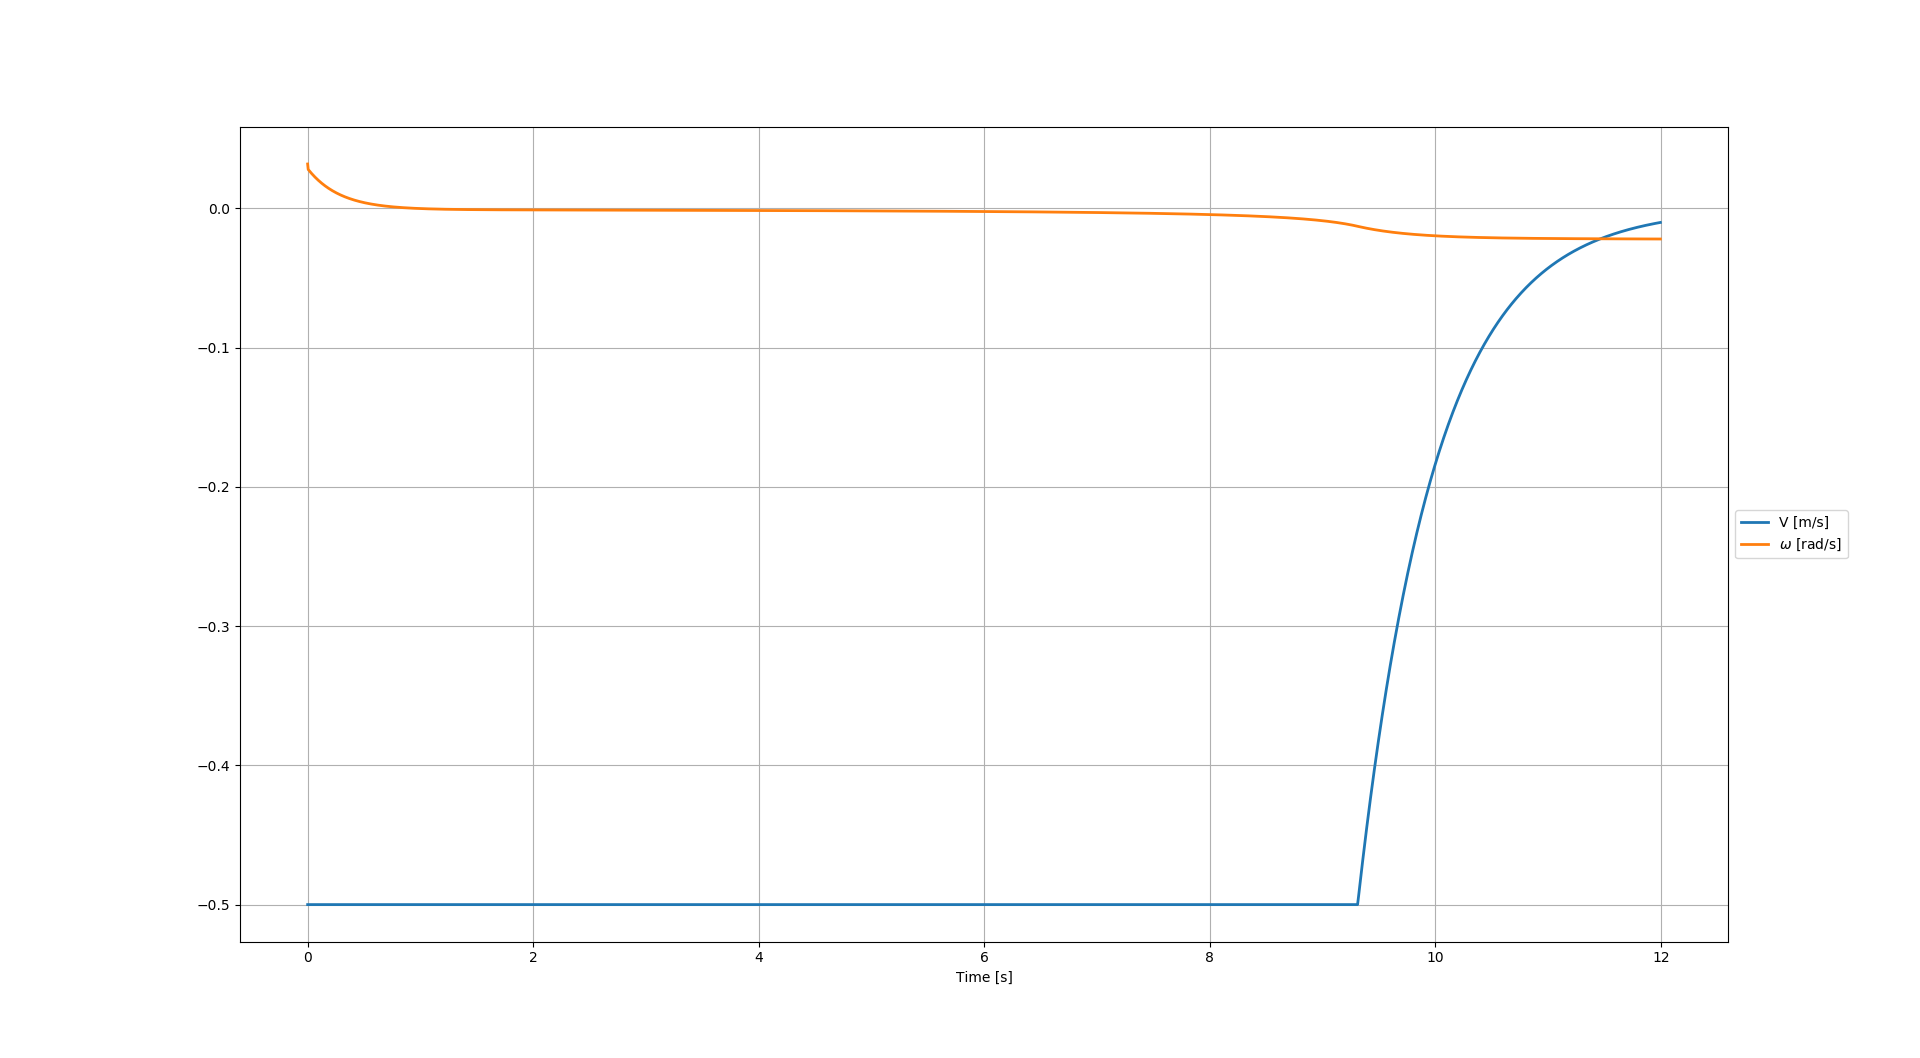
\includegraphics[width=\textwidth]{../Figures/hw1_3_ii_b_reverse.png}
	\end{figure}
	\begin{figure}[H]
		\centering
		\title{\bf Parallel Trajectory}
		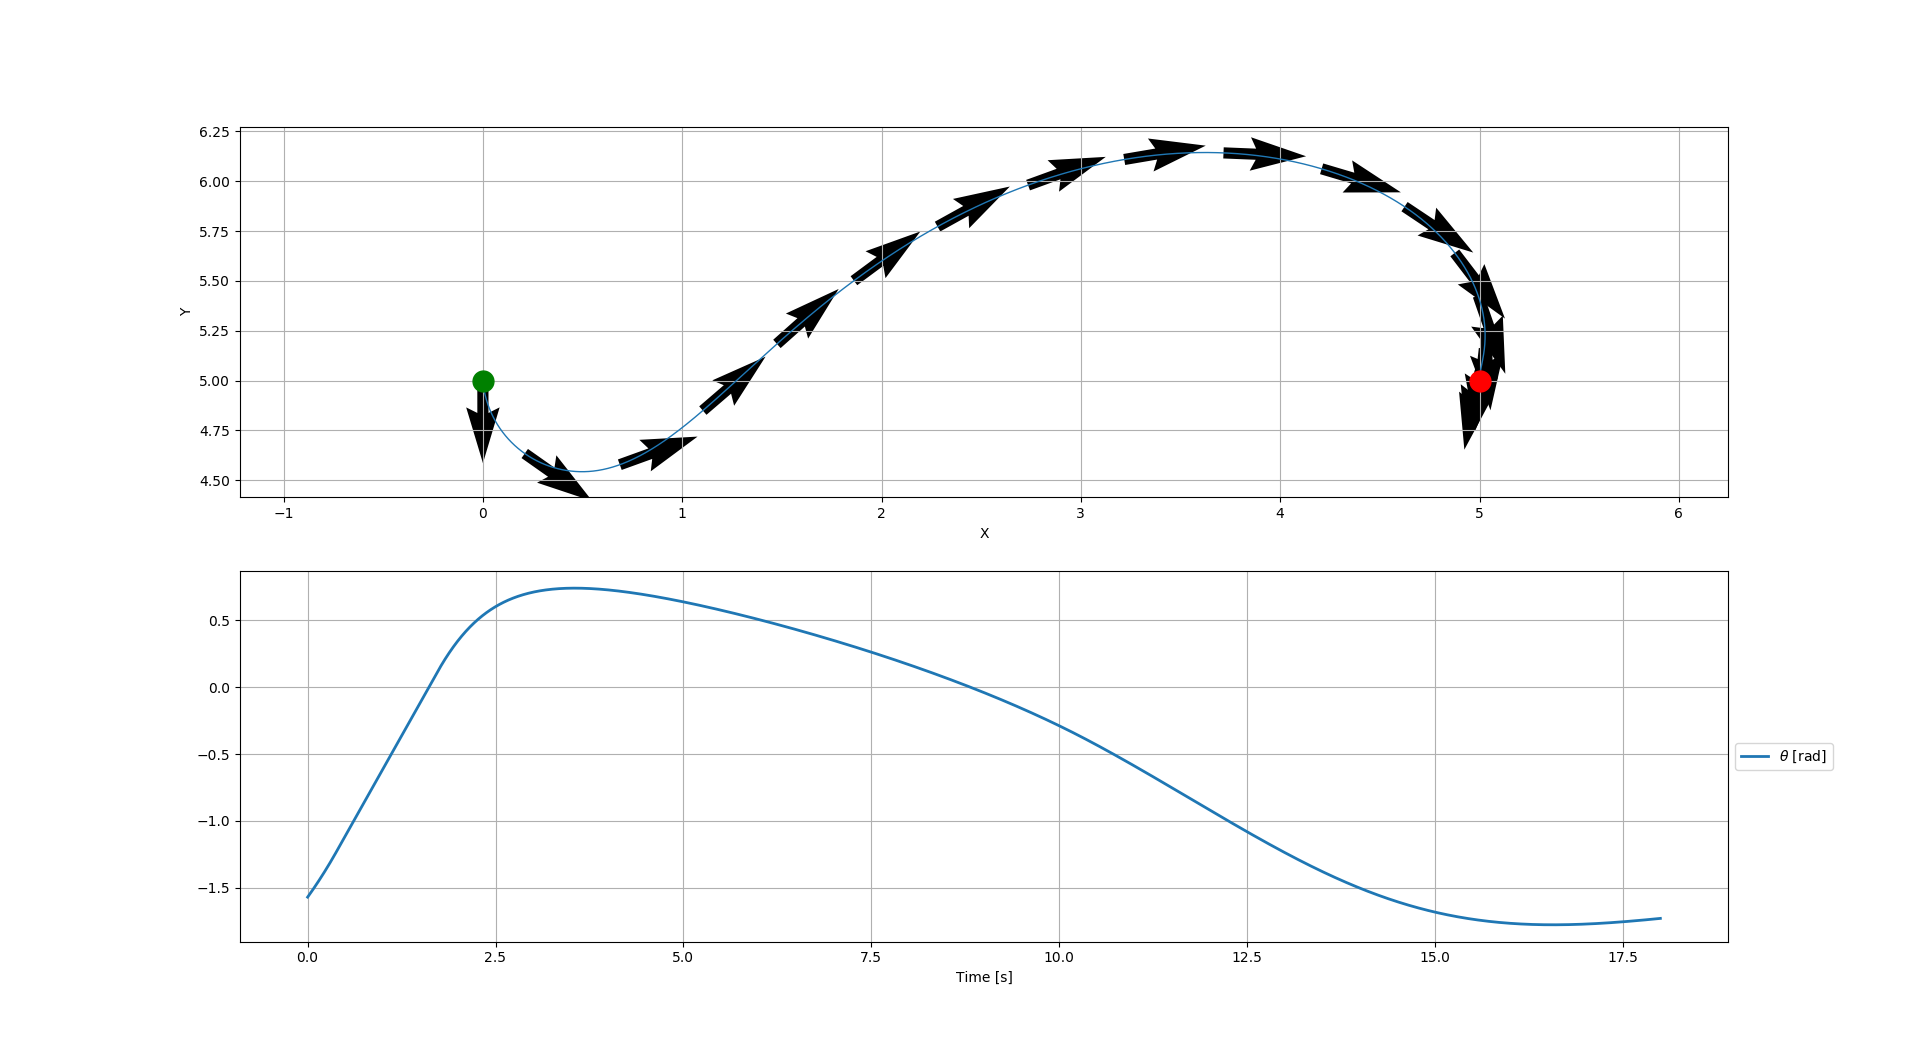
\includegraphics[width=\textwidth]{../Figures/hw1_3_ii_a_parallel.png}
	\end{figure}
	\begin{figure}[H]
		\centering
		\title{\bf Parallel Control}
		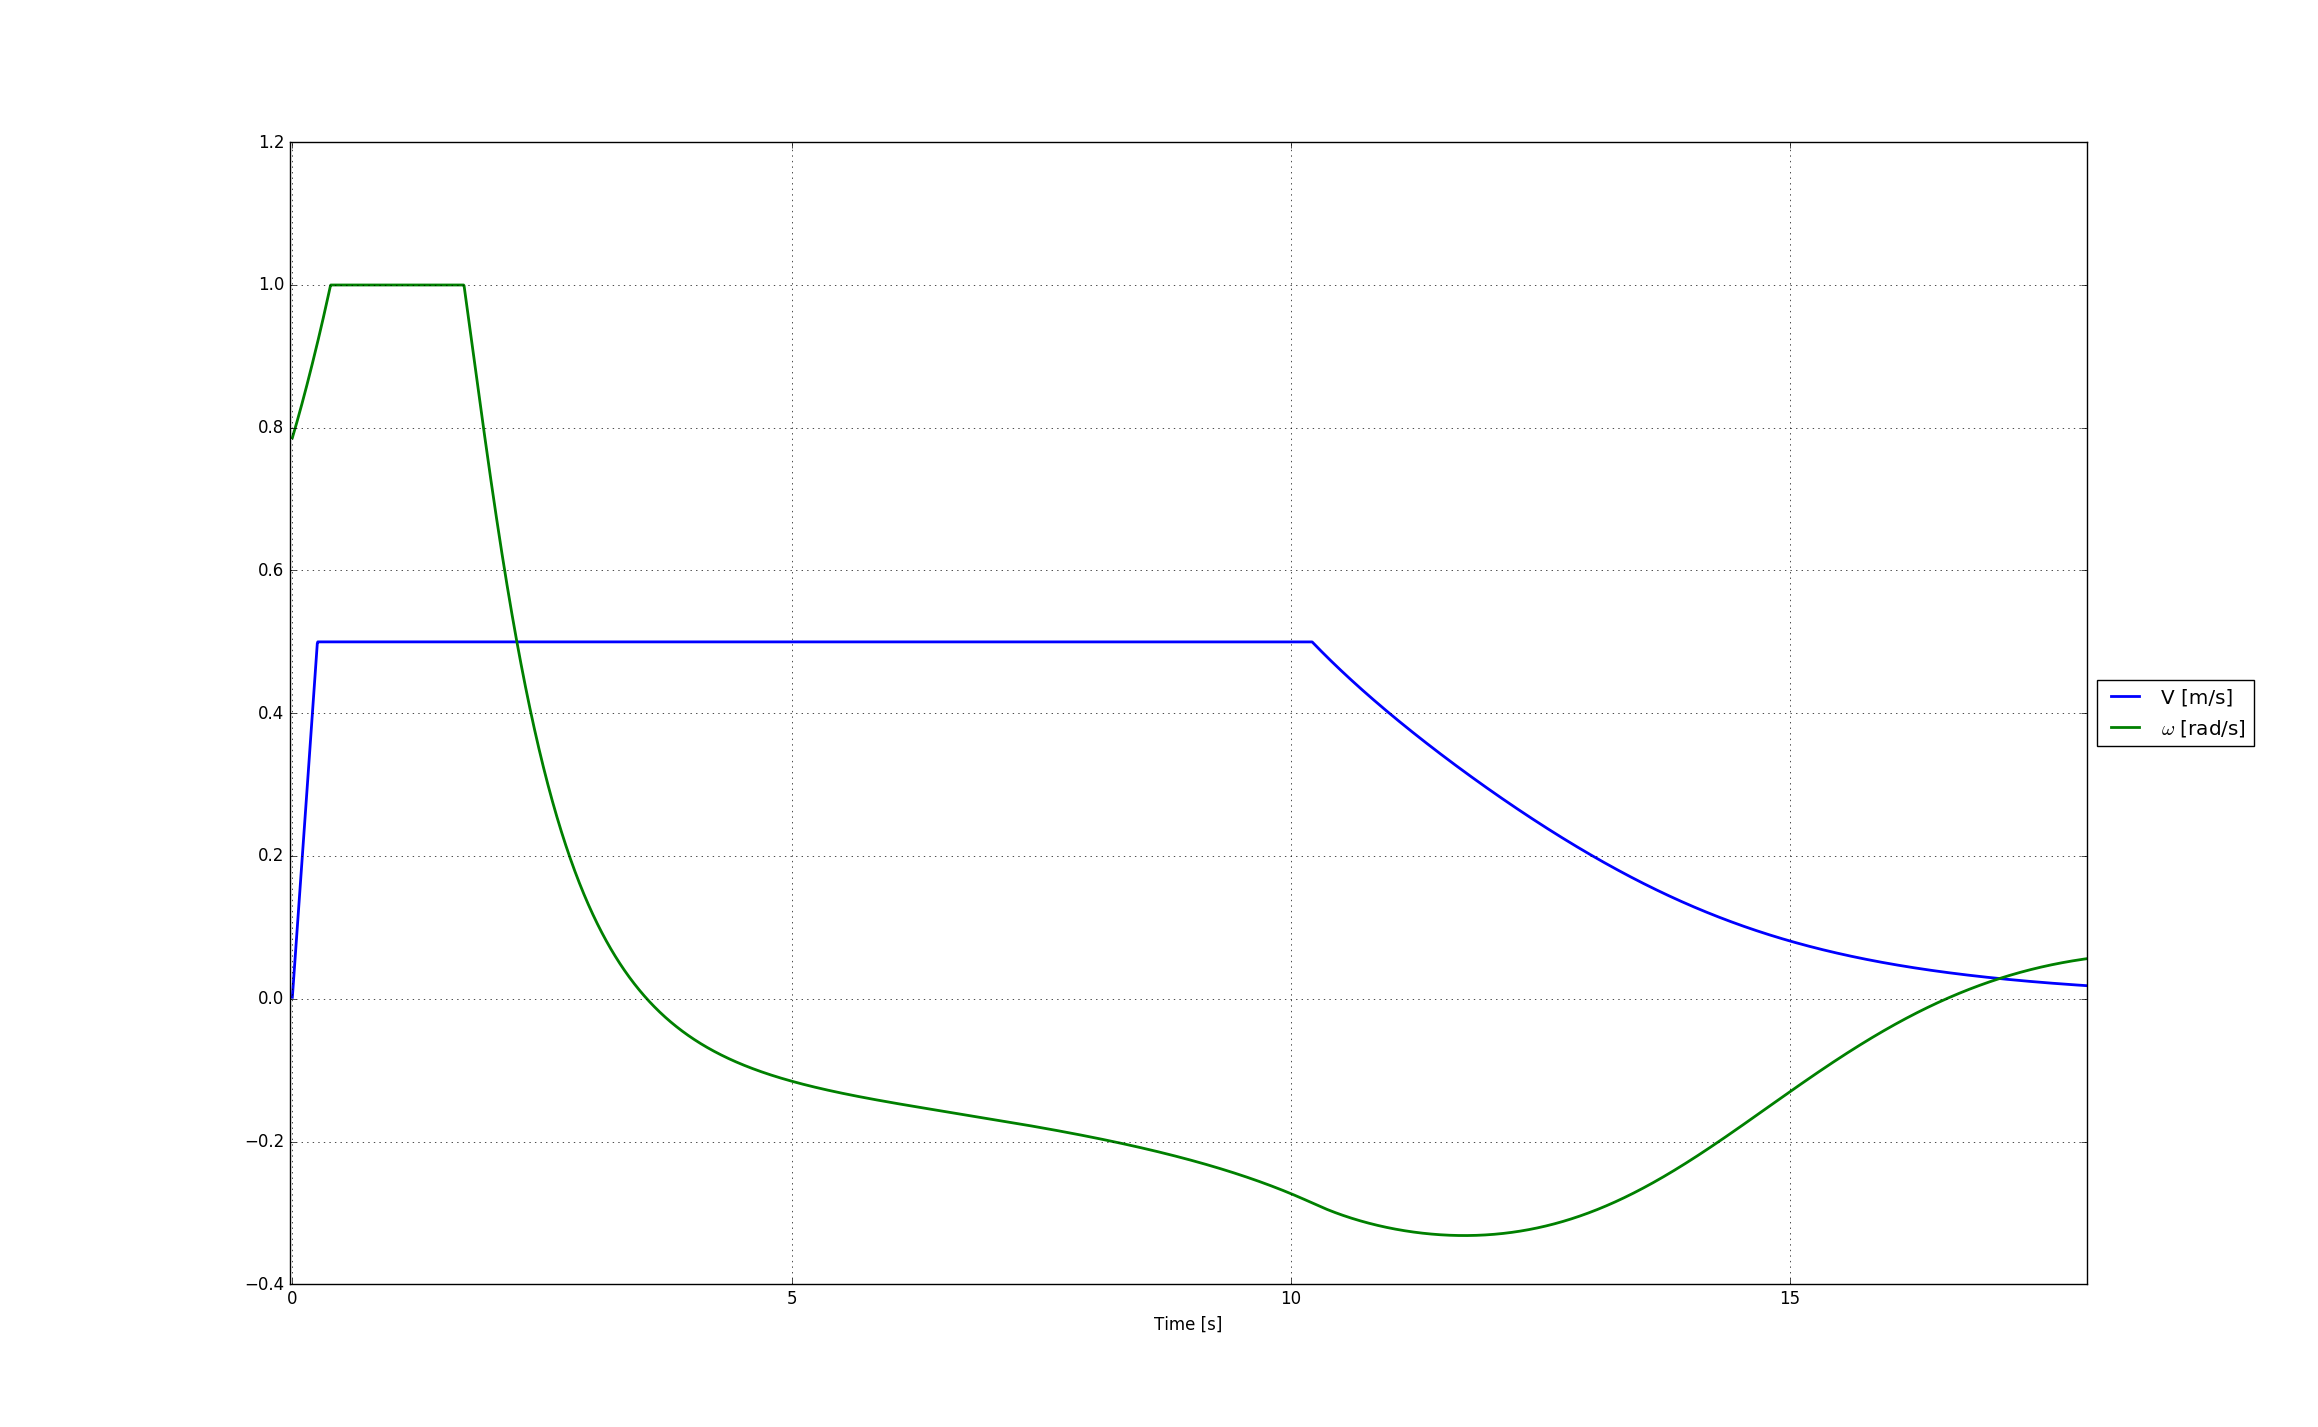
\includegraphics[width=\textwidth]{../Figures/hw1_3_ii_b_parallel.png}
	\end{figure}
\end{enumerate}

\section{Closed-loop Control II}
\begin{enumerate}
	\item We wish to implement the virtual control law
	\begin{align*}
		u_1 &= \ddot x_d + k_{px}(x_d - x) + k_{dx}(\dot x_d - \dot x) \\
		u_2 &= \ddot y_d + k_{py}(y_d - y) + k_{dy}(\dot y_d - \dot y)
	\end{align*}
	with control gains $k_{px}, k_{py}, k_{dx}, k_{dy} > 0$ and desired (differential flatness) trajectory $(x_d,y_d)$. In Problem 2, part (ii), we showed that for a given state $\mathbf{x} = (x,y,\theta)$,
	\begin{equation}\label{eqn:4_1_system}
		\left(\begin{array}{c}
		a \\
		\omega
		\end{array}\right) =
		\left(\begin{array}{c}
		\dot V \\
		\omega
		\end{array}\right) =
		\left(\begin{array}{c}
		u_1\cos(\theta) + u_2\sin(\theta) \\
		\frac{1}{V}(-u_1\sin(\theta) + u_2\cos(\theta))
		\end{array}\right)
	\end{equation}
	where the virtual controls are $(u_1,u_2) = (\ddot x, \ddot y)$.
	\item See submitted code. We assume the virtual control law is implemented at a high enough frequency that the state can be treated as constant. Furthermore, at each step $t$, we consider the current velocity to be that commanded at $t-1$, i.e.,
	\[
		\dot x_t = V_{t-1}\cos(\theta), \quad \dot y_t = V_{t-1}\sin(\theta).
	\]
	Using this, we can calculate $(u_1,u_2)$ and plug into (\ref{eqn:4_1_system}) to get the current acceleration, $a_t = \dot V_t$. We then apply the Euler method to update
	\[
		V_t = V_{t-1} + (dt)\dot V_t \quad \mbox{where $dt$ is the timestep}.
	\]
	If $V_t \approx 0$, we reset it to the nominal (desired) velocity $V_d = \sqrt{\dot x_d^2 + \dot y_d^2}$ according to the robot kinematic model. Finally, we calculate $\omega$ from (\ref{eqn:4_1_system}).
	\item See submitted code.
	\item See submitted code. For this simulation, we set $(k_{px}, k_{py}, k_{dx}, k_{dy}) = (1,1,0.5,0.5)$ and reset to the nominal velocity whenever $|V_t| \leq \epsilon = 10^{-5}$. The following plots were made with initial conditions $(x_0,y_0,\theta_0) = (0,0,-\pi/2)$.
	\begin{figure}[H]
		\centering
		\title{\bf Trajectory $(x(t), y(t))$}
		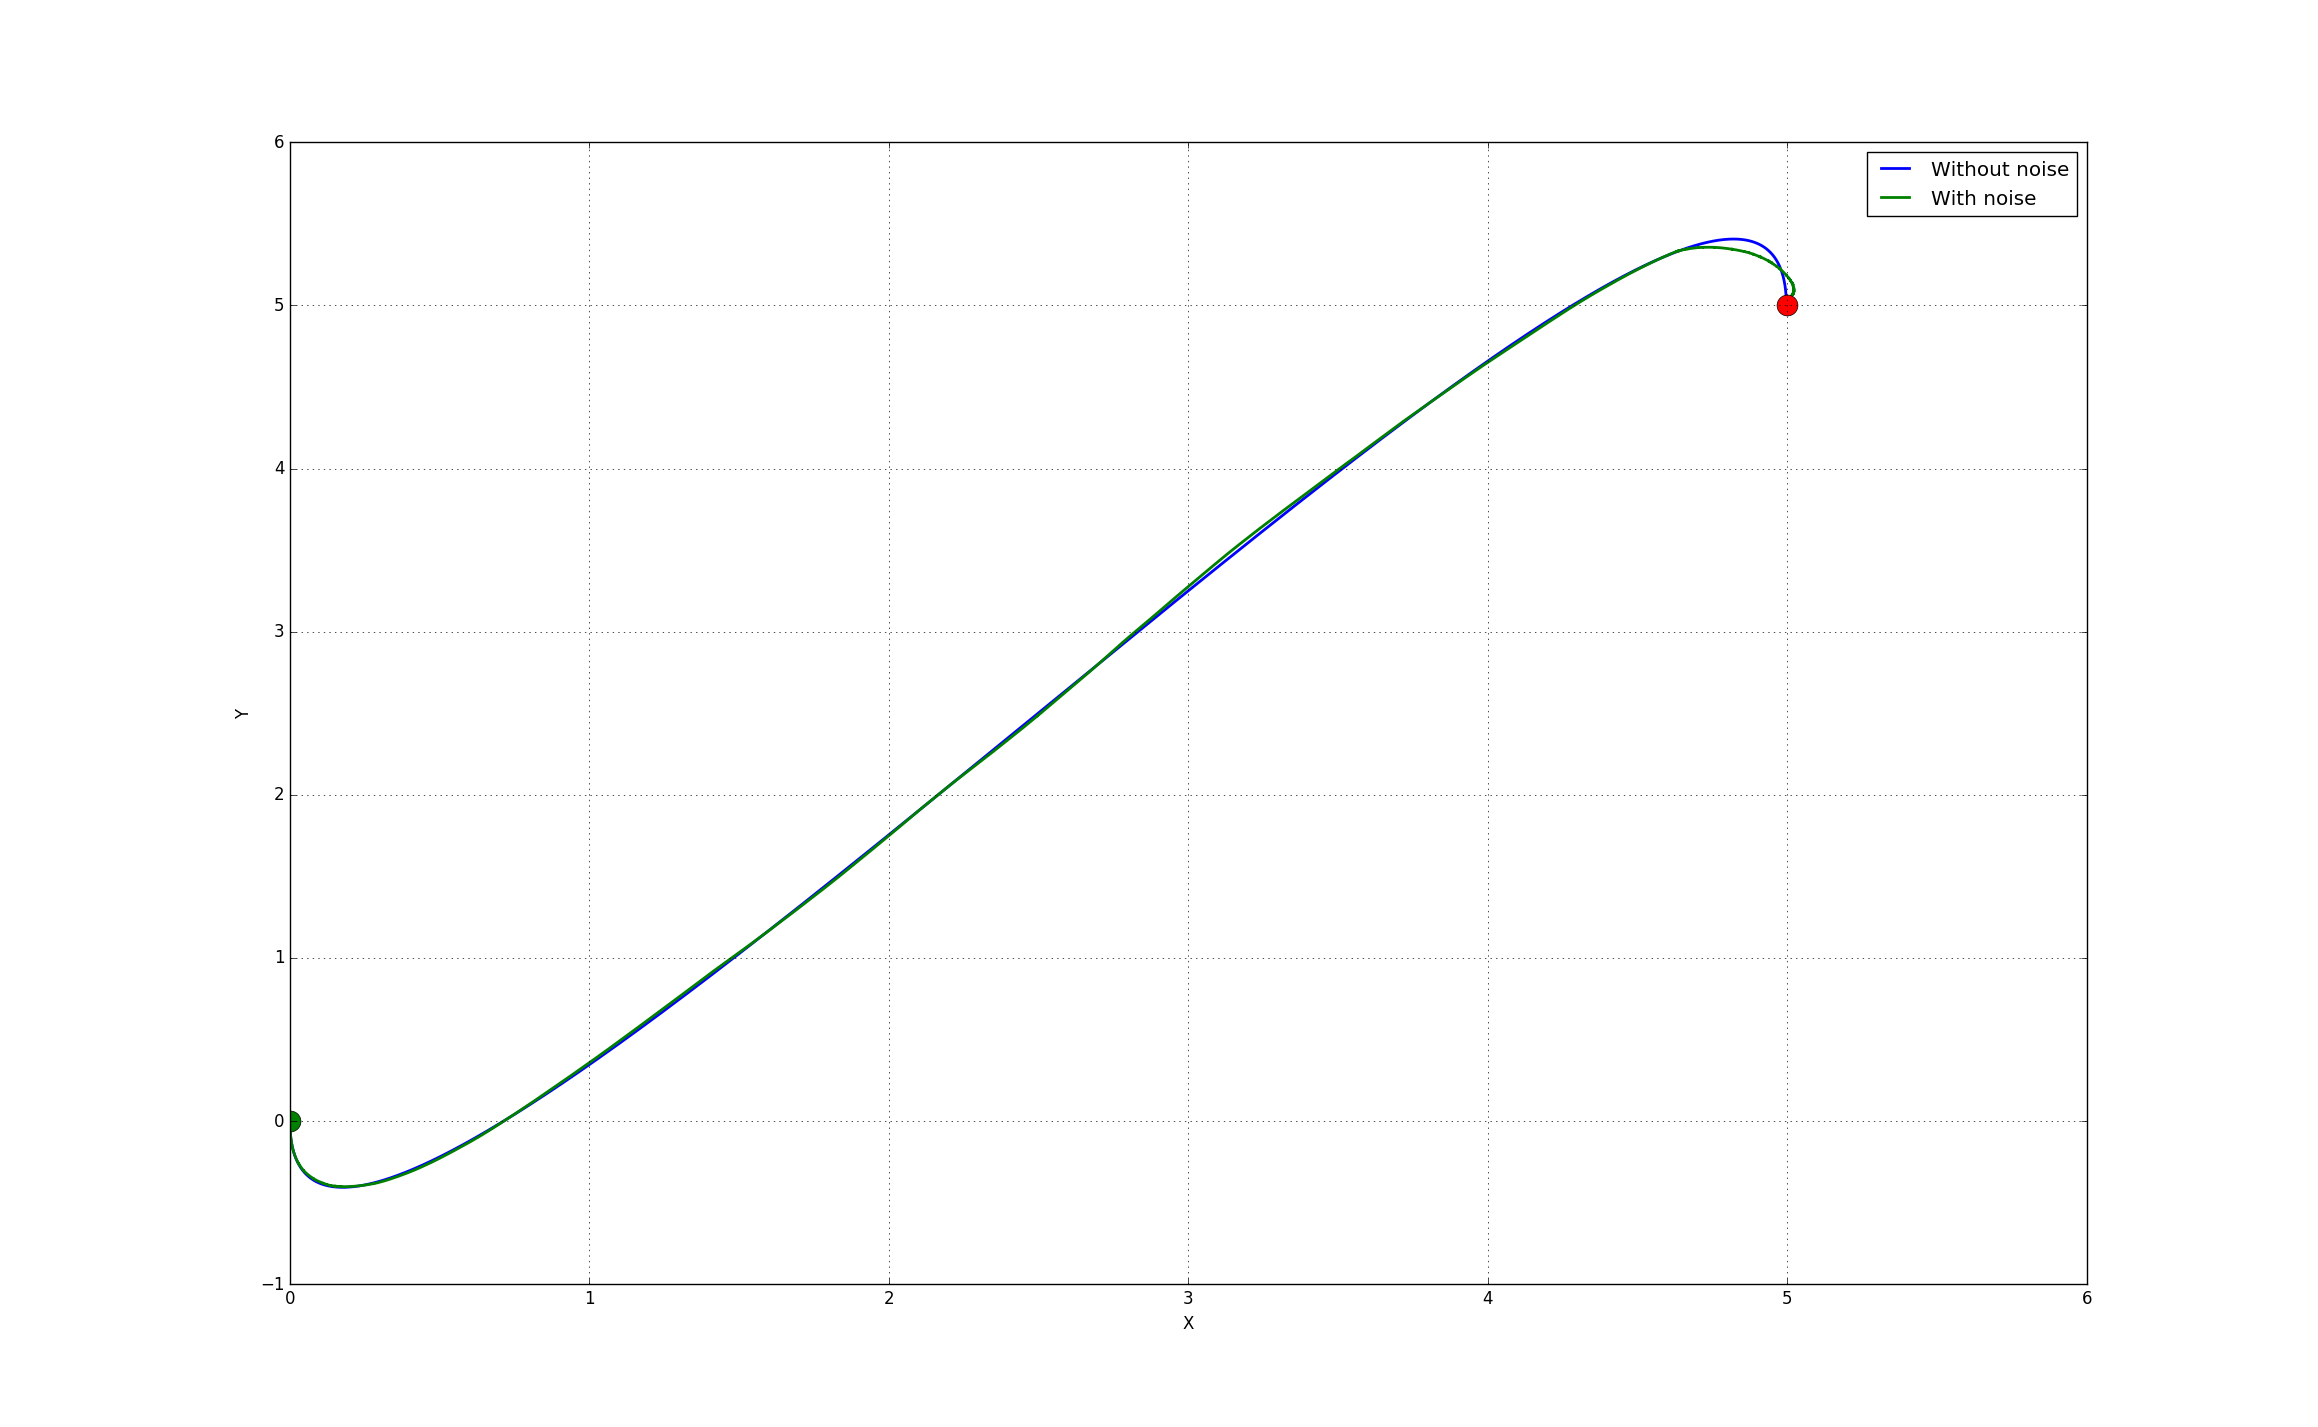
\includegraphics[width=\textwidth]{../Figures/hw1_4_iv_traj.png}
	\end{figure}
	\begin{figure}[H]
		\centering
		\title{\bf History of $V$ and $\omega$}
		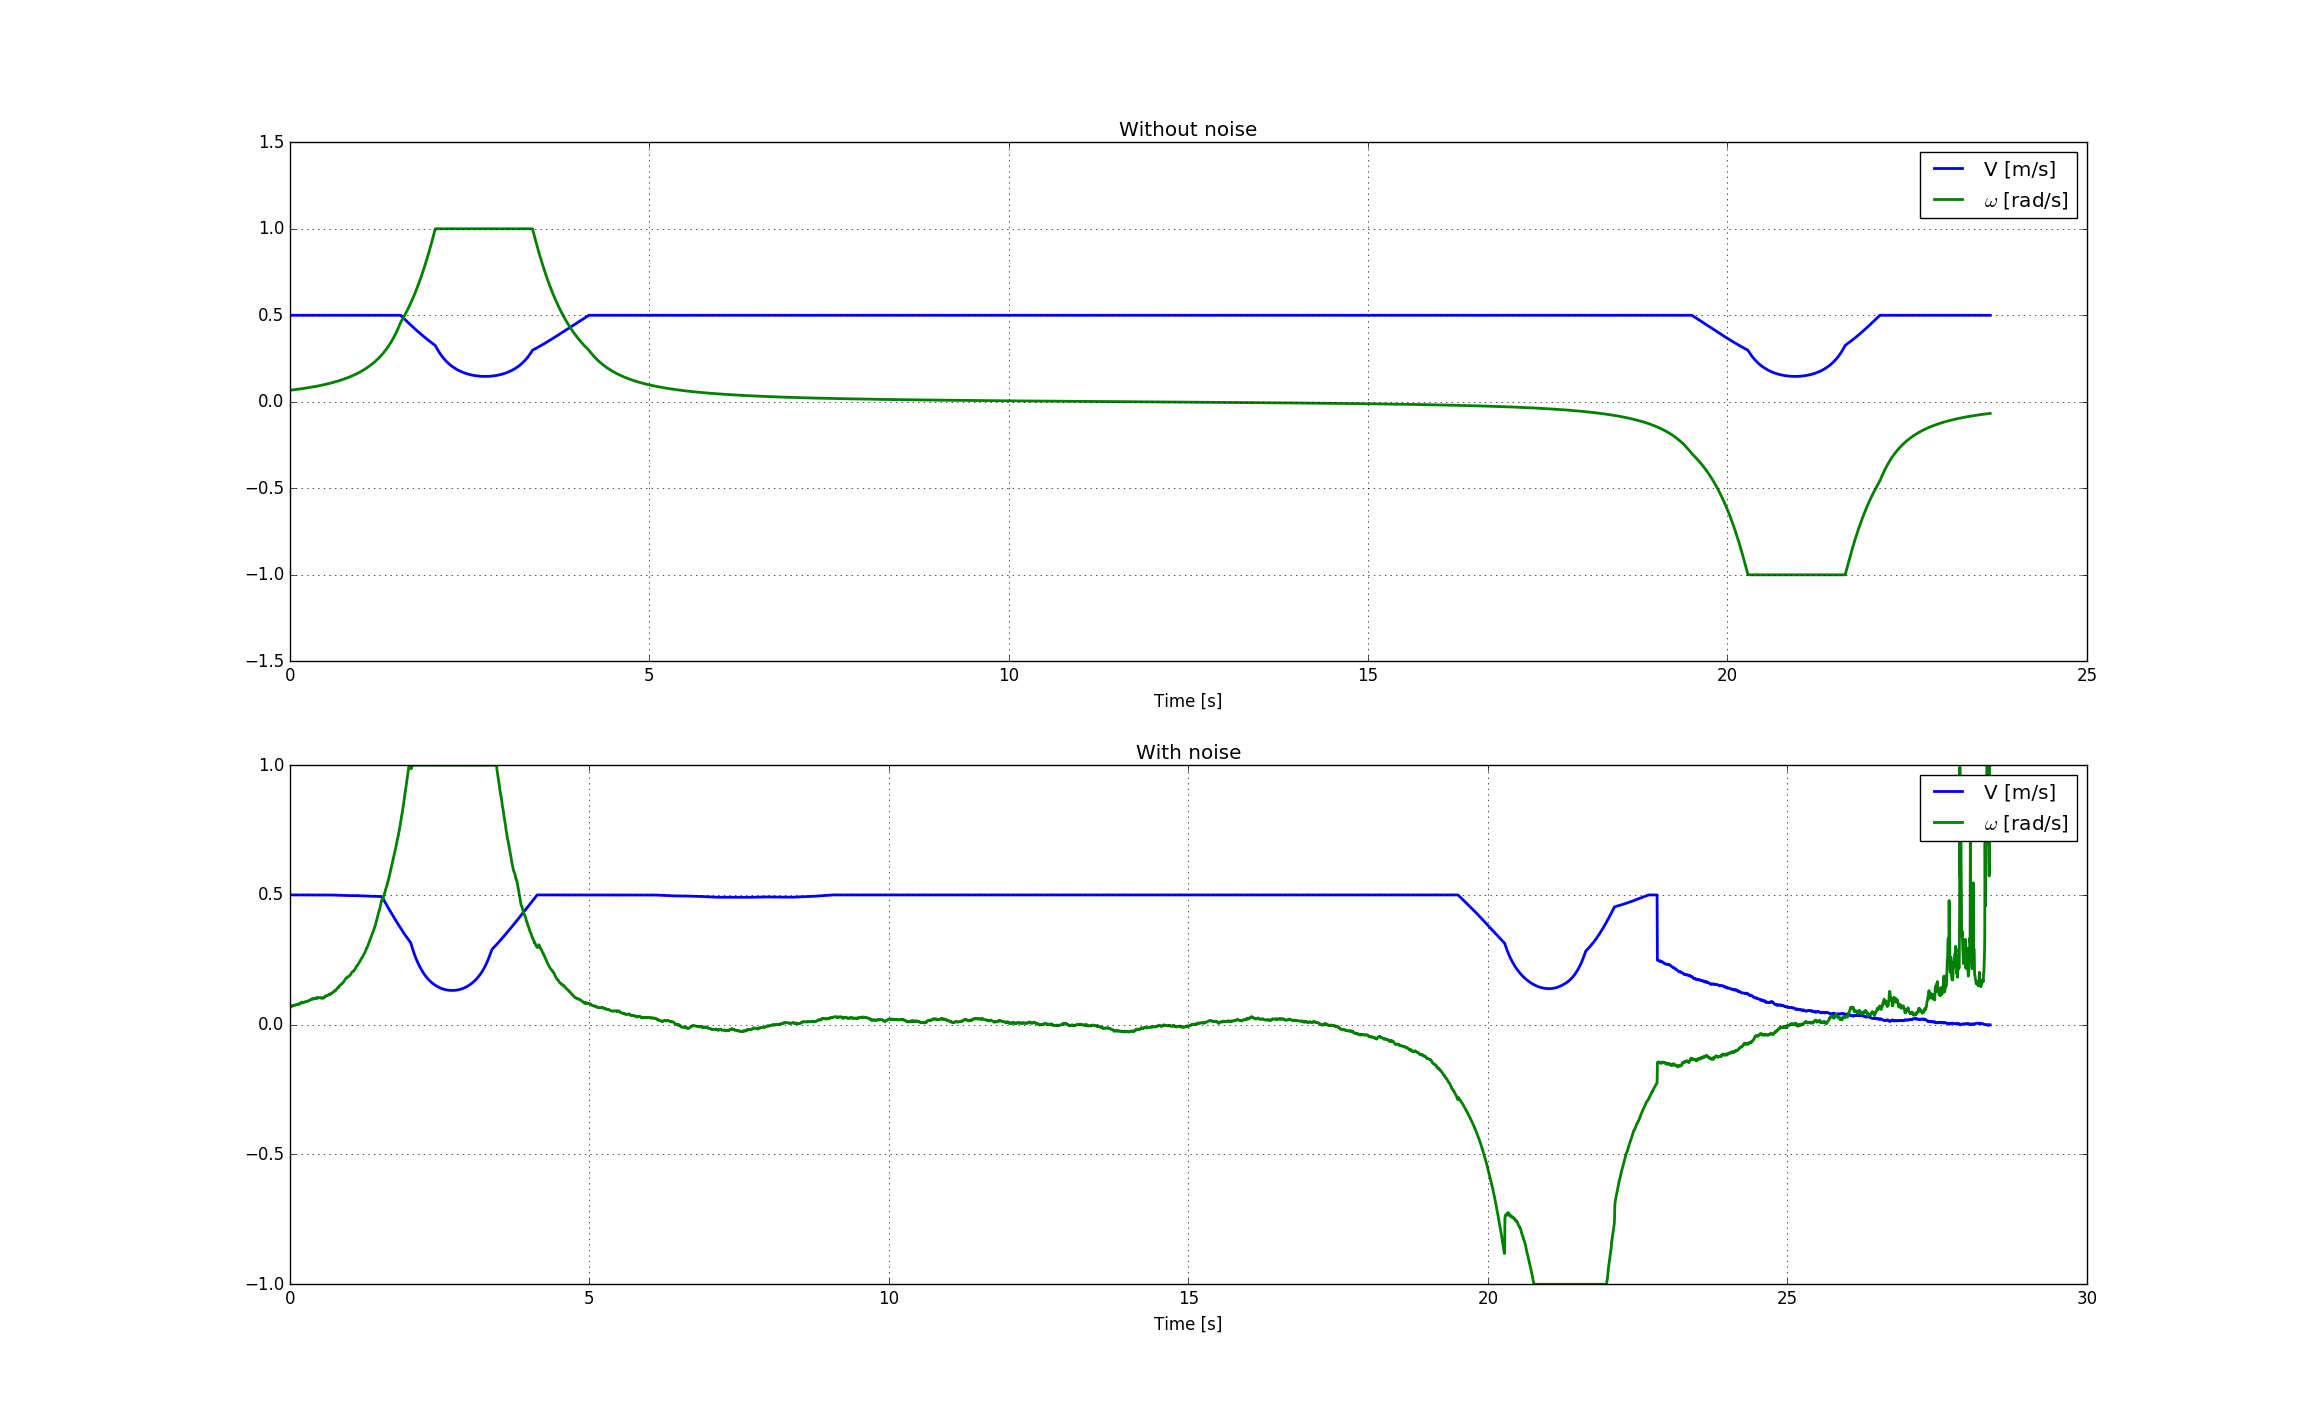
\includegraphics[width=\textwidth]{../Figures/hw1_4_iv_ctrl.png}
	\end{figure}
\end{enumerate}

\section{Robot Operating System}
\begin{enumerate}
	\item See submitted code.
	\item \verb|rosbag play filename.bag|
	\item See submitted code.
\end{enumerate}
\end{document}